%!TEX root = ../lections.tex
\section{Введение}

Курс \textbf{механики сплошных сред} (далее \textbf{\textbf{МСС}}) является одним из разделов цикла теоретической физики.  Так, в знаменитом курсе теоретической физики Л.Д.Ландау и Е.М.Лифшица  ему посвящено два достаточно объемных тома (объем свыше 1000 страниц).

Наш курс для радиофизиков – он существенно меньше, чем курсы на специализированных факультетах. Он рассчитан на радиофизиков, несколько больший объем в нем занимают волновые процессы.

Следует отметить, что исходные уравнения механики сплошных сред существенно сложнее чем уравнения электродинамики, где базовыми являются линейные уравнения Максвелла. В тоже время, в этих курсах возникают одинаковые уравнения, это одна из причин почему курсу читаются параллельно. В этих курсах большую роль играют формулы векторного анализа.

История развития \textbf{МСС} полностью подтверждает наличие тесной связи между становлением науки и запросами практики.  
\textbf{МСС} -- одна из древнейших наук. Ее зарождение идет еще в античной древности.

Фамилии (но не годы жизни) знают все. Это:
\begin{itemize}
	\setlength\itemsep{-0.4em}
	\item Аристотель (384-322 г.г. до н.э)
	\item Архимед (287-212 г.г. до н.э) – закон Архимеда
\end{itemize}
	Средние века:
\begin{itemize}
	\setlength\itemsep{-0.4em}
	\item Галилей (1564-1642)
	\item Паскаль (1623-1662) 
	\item Леонардо де Винчи (1452-1519)
	Это и летательные аппараты, закон Паскаля для давления, наблюдение гидродинамической турбулентности.
	\item Гюйгенс (1629-1695)
	\item Ньютон (1642-1727). В своих знаменитых \emph{<<Началах>>} он приводит теоретический вывод квадратичного закона сопротивления. Именно из законов Ньютона было проведено обобщение на сплошные среды и родилась новая наука <<гидромеханика>>.
\end{itemize}
Это два академика Российской академии наук
\begin{itemize}
	\setlength\itemsep{-0.4em}
	\item Леонард Эйлер (1707-1789) – уравнение Эйлера
	\item Даниил Бернулли (1700-1782) -  уравнение Бернули
	\item Даламбер (1717-1783) – парадокс
\end{itemize}
Начало 19 века:
\begin{itemize}
	\setlength\itemsep{-0.4em}
	\item Лагранж (1736-1813)
	\item Коши (1789-1857)
\end{itemize}
Вязкая жидкость:
\begin{itemize}
	\setlength\itemsep{-0.4em}
	\item Анри Навье  (1785-1863)
	\item Стокс (1819-1903) – уравнение Навье-Стокса
\end{itemize}
Эксперименты с жидкостью:
\begin{itemize}
	\setlength\itemsep{-0.4em}
	\item Ж. Пуазейль (1799-1869)
\end{itemize}
Основы теории турбулентности:
\begin{itemize}
	\setlength\itemsep{-0.4em}
	\item Осборн Рейнольдс (1842-1912)
	\item Н.Е.Жуковский (1847-1921) Обтекание крыла, присоединённый вихрь, подъемная сила
	\item С.А.Чаплыгин (1869-1942)
	\item Морис Мари Альфред Куэтт  (1858-1943) – течение Куэтта
\end{itemize}
Теории турбулентности и теория устойчивости:
\begin{itemize}
	\setlength\itemsep{-0.4em}
	\item Людвиг Прандтль  (1875-1953)
	\item Теодор Карман (1881-1963)
\end{itemize}

Практически все эти фамилии будут встречаться в нашем курсе – их именами названы законы \textbf{МСС}.

В наше время бурное развитие получила вычислительная \textbf{МСС}. Так, не один новый самолет не получит разрешение на эксплуатацию, если не будет построена его математическая модель, включающая процессы самолета  обтекания потоком.

Что же включает современная \textbf{МСС}? Книга академика Л.Седова <<Краткое перечисление современных проблем>> включает 21 пункт и занимает 4 страницы. Здесь мы приведем лишь те, которые тесно связаны с предприятиями и НИИ Нижнего Новгорода, и где работают выпускники радиофака.

\begin{enumerate}
	\item Изучение движения жидкости и газа – движение самолетов, вертолетов, подводных лодок.  Возникновение турбулентных следов за объектами. Излучение звука винтами и турбулентными струями. ИПФ РАН, ОКБМ.
	\item Движение жидкости и газа в трубах. Взаимодействие волн в оболочках. ИПФ РАН, ОКБМ.
	\item Волновые движения в жидкостях и газах
	\begin{itemize}
		\item Волны в твердых телах.  Акустическая диагностика, взаимодействие с электромагнитными волнами – линии задержки на ПАВ (радиоэлектронной комплекс НО)
		\item Волны на поверхности моря и внутренние волны, их нелинейное взаимодействие. Обнаружение ПЛ по изменению характеристик поверхностного волнения.
		\item Волны в каналах, реках. Генерация цунами и  набег волн цунами на берег.
		\item Сейсмические процессы, нелинейная сейсмодиагностика.
		\item Звуковые волны,  гидроакустика, акустика океана
	\end{itemize}
	\item Теория турбулентности – гравитационная неустойчивость
	\item Биологическая механика, движение крови в сосудах, диагностика на различных типах волн – сдвиговые волны
\end{enumerate}
Пример – \textbf{Институт прикладной физики РАН}, один из крупнейших институтов Российской академии наук.
Филиалы:
\begin{itemize}
	\item \textbf{Институт физики микроструктур} РАН
	\item \textbf{Институт проблем машиностроения} РАН
\end{itemize}

\textbf{Федеральное государственное бюджетное научное учреждение <<Федеральный исследовательский центр Институт прикладной физики Российской академии наук>> (ИПФ РАН)} был создан на базе нескольких отделов Научно-исследовательского радиофизического института (НИРФИ) Минвуза РСФСР в апреле 1977 года. Основатель и директор института на протяжении первых 25 лет его работы — академик А. В. Гапонов-Грехов, с 2003 по 2015 год институт возглавлял академик А. Г. Литвак, с 2015 года до своего избрания президентом РАН в 2017 году директором института был академик А. М. Сергеев. С октября 2017 г. временно исполняющим обязанности директора ИПФ РАН назначен член-корреспондент РАН Г.Г. Денисов.

\subsection{Основные допущения \textbf{МСС}}
Вещество можно рассматривать как непрерывную сплошную среду, пренебрегая его молекулярным строением. И однвременно считаем непрерывным распределение всех характеристик жидкости (плотность, скорость, температура, $\ldots$).

Это означает, что всякий малый элемент жидкости или газа содержит большое число молекул(или других частиц ). То есть когда мы говорим о бесконечно малом элементе жидкости, то везде мы подразумеваем,  что \emph{<<физически>>} бесконечно малый объем мал по сравнению с размерами тел, но велик по сравнению с межмолекулярными расстояниями.

Это позволяет применить в \textbf{МСС} хорошо разработанный для непрерывных функций аппарат высшей математики.

Нетривиальный пример – \textbf{крупномасштабная структура Вселенной.}

Описание развития крупномасштабной структуры  уравнениями гидродинамики газа гравитационно взаимодействующих частиц. \emph{<<Физически>>} бесконечно малый объем – объем в котором содержится много галактик.

Существующие на данный момент крупномасштабные образования возникли из-за малых начальных возмущений плотности за счет гравитационной неустойчивости. Обычная материя (атомов различных веществ) (4\%), Темная материя неизвестной физической природы (cold dark matter) (23\%). Темная энергия (dark energy) (73\%), которая играет антигравитационную роль в процессе формирования Вселенной.

Плотность темного вещества в 6–7 раз превосходит плотность барионов, и поэтому рост неоднородностей определяется в основном темным веществом. Именно рост неоднородностей в темном веществе и ответственен за формирование крупномасштабных структур. Барионная компонента просто следовала за эволюцией темного вещества.

В космологии понятие крупномасштабной структуры относится к распределению галактик и массы темного вещества (на масштабах от одного до нескольких сотен мегапарсек). Современная теория объясняет формирование крупномасштабной структуры Вселенной как следствие роста исходных слабых флуктуаций плотности вещества за счет гравитационной неустойчивости. При этом формирование ярко выраженных элементов структуры происходит на нелинейной стадии. Именно поэтому процесс формирования крупномасштабной структуры принято иногда гравитационной турбулентностью.

Наиболее очевидный путь преодоления сложности учета законов нелинейной эволюции гравитационной неустойчивости на поведение поля плотности вещества состоит в численном моделировании трехмерного движения $N$ гравитационно взаимодействующих частиц. Альтернативой являются приближенные аналитические решения некоторых уравнений в частных производных, адекватно описывающих рост флуктуаций неоднородной плотности вещества в расширяющейся Вселенной. Первый из этих подходов был предложен Зельдовичем в 1970 году.

Второй аналитический подход к проблеме описания формирования крупномасштабной структуры Вселенной \cite{a1} базируется на векторном уравнении Бюргерса. В данном подходе многопотоковое движение гравитационно взаимодействующих частиц в особенностях, приводящее к их локализации, моделируется вязким слагаемым в уравнении Бюргерса. В предельном случае исчезающе малой вязкости это эквавалентно слипанию частиц и поэтому данный подход часто называют приближением слипания - adhesion model (см., например, \cite{a2,a3,a4,a5}. 

% Adhesion model Модель Зельдовича-Гурбатова-Саичева
Предельная версия модели слипания естественным образом описывает характерную мозаичную структуру распределения вещества во Вселенной. Основные элементы <<мозаики>> в трехмерном пространстве (вершины, ребра, грани и внутренности ячеек) могут быть ассоциированы с наблюдаемыми структурами трехмерного распределения галактик (компактные скопления галактик, филаменты – цепочки галактик, поверхности со сравнительно высокой плотностью галактик, и темные области между ними, бедные галактиками).

Сама эволюция крупномасштабной структуры Вселенной может трактоваться как непрерывый процесс транспортировки вещества преимущественно из объектов большой размерности к объектам мозаичной структуры, обладающим меньшей размерностью. К примеру, вещество из внутренних ячеек мозаичной структуры (трехмерных объектов) перетекает в ее грани (квазидвумерные объекты), а из них в ребра и вершины мозаичной структуры. В то же время, сами ячейки участвуют в непрерывном движении, деформации и поглощении одних ячеек другими.

\begin{figure}[H]
	\centering
	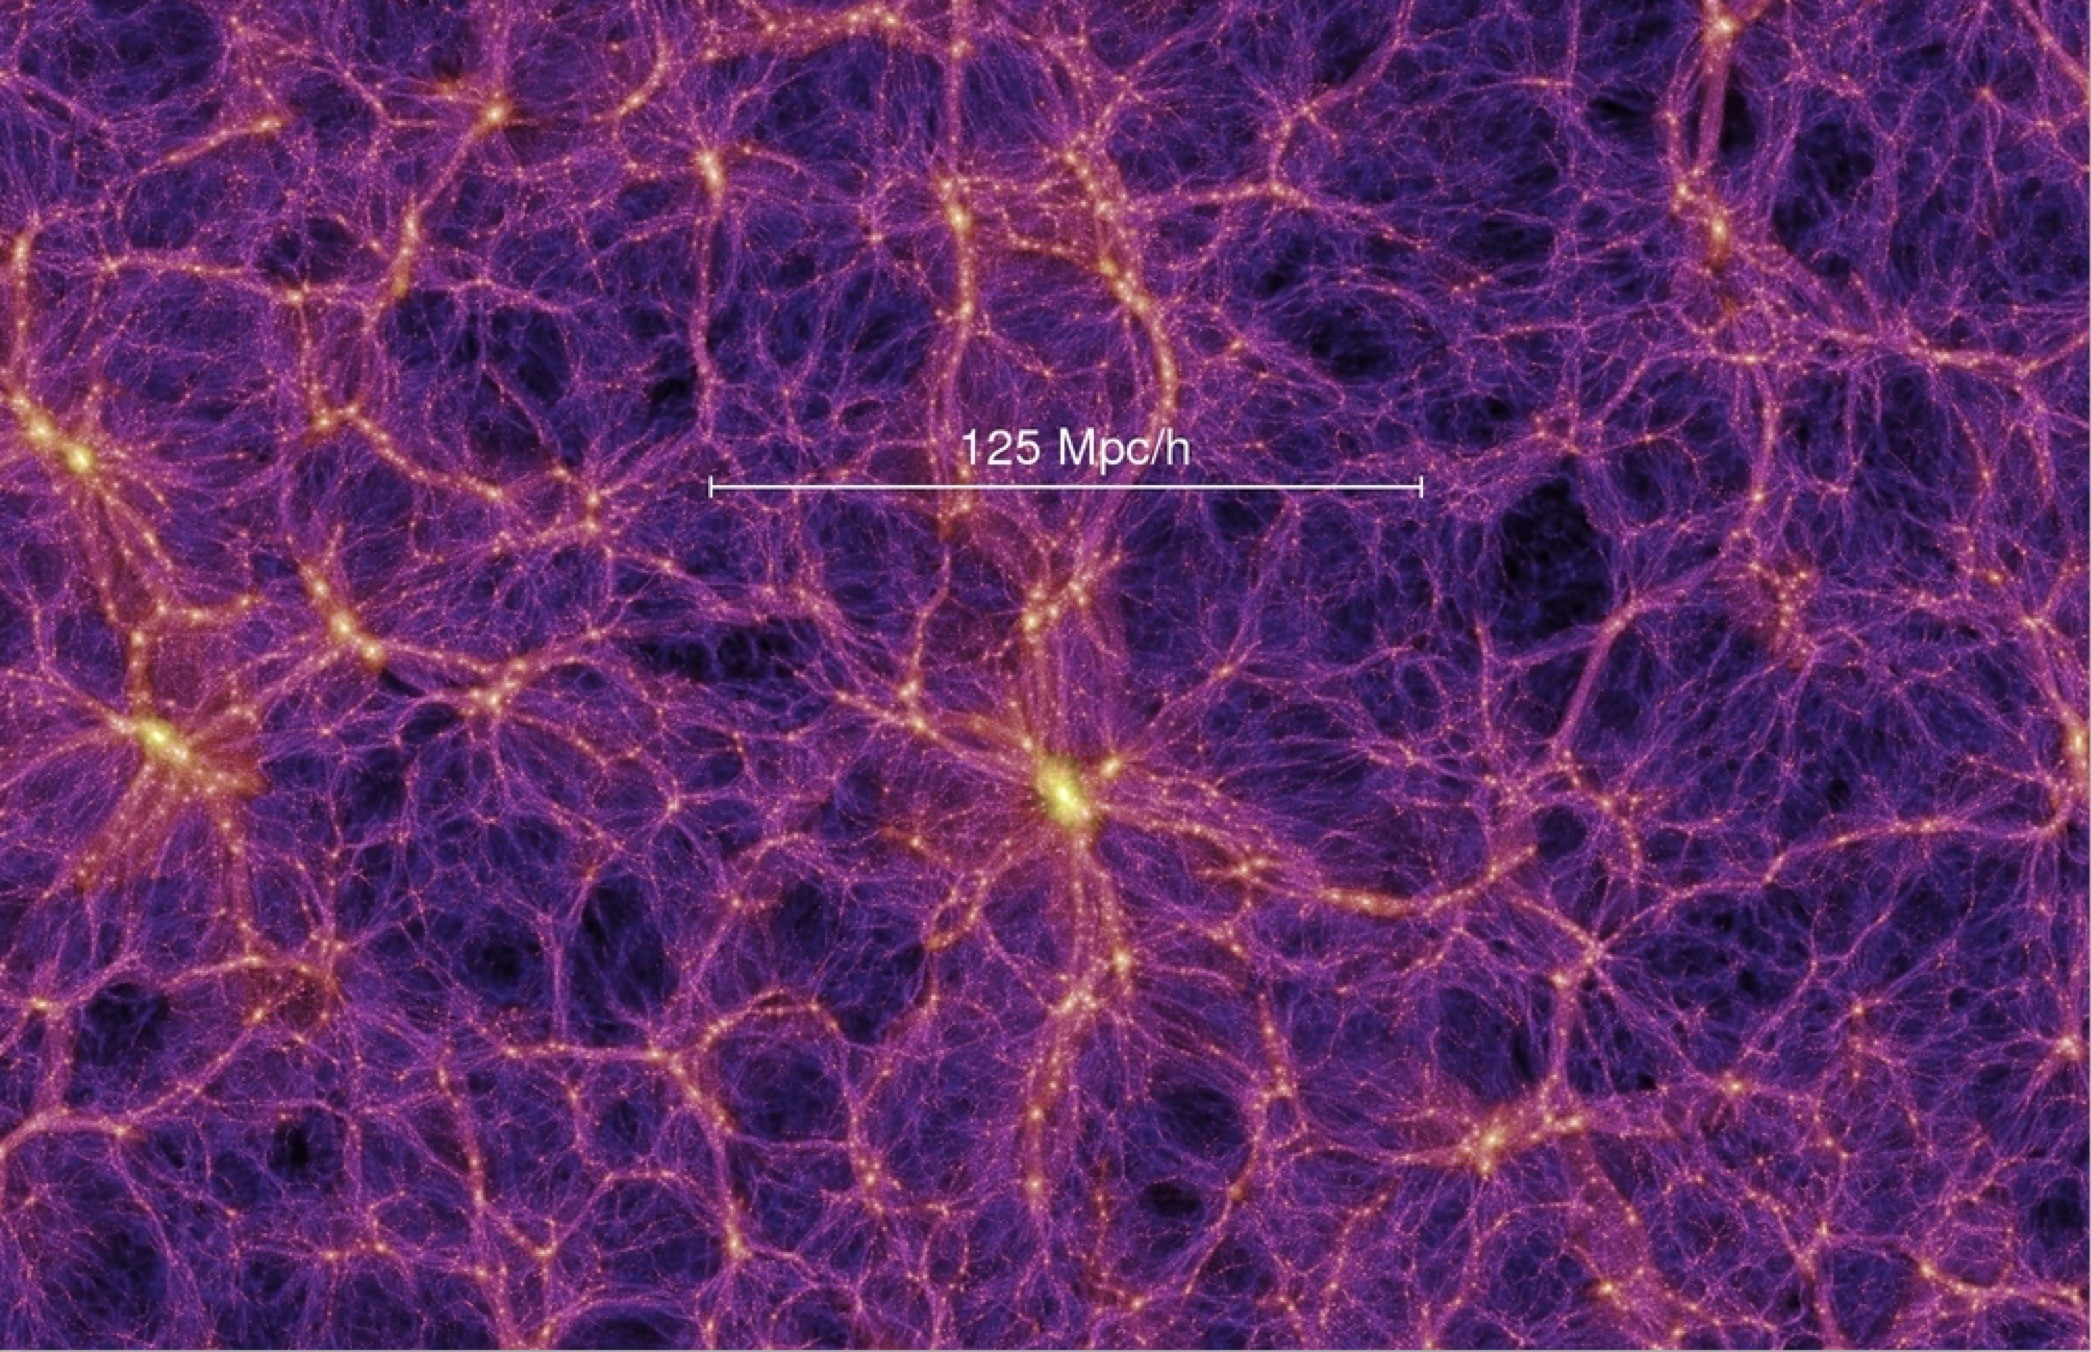
\includegraphics[width=.6\linewidth]{photo/1.jpg}
	\caption{Крупномасштабная структура Вселенной}
	\label{fig:figure1}
\end{figure}
\begin{figure}[H]
	\centering
	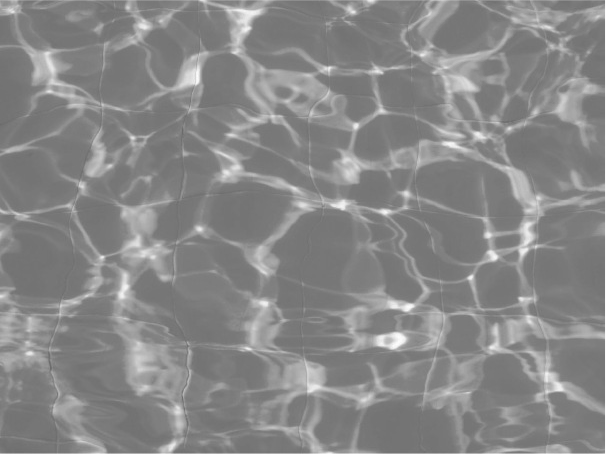
\includegraphics[width=.6\linewidth]{photo/2.png}
	\caption{Система каустик на дне бассейна}
	\label{fig:figure2}
\end{figure}
В заключение отметим, что результаты динамического моделирования в рамках приближения слипания можно посмотреть на Youtube (\textbf{The Sticky Geometry of the Cosmic Web, version 2.01})

\url{https://www.youtube.com/watch?v=wI12X2zczqI}

Результаты прямого численного моделирования (N-body simulation) можно также  посмотреть на Youtube

Двухмерный случай:

\url{https://www.youtube.com/watch?v=nHvcqV92oqY}

\url{https://www.youtube.com/watch?v=74IsySs3RGU}

Трехмерный случай

\url{https://www.youtube.com/watch?v=eDGtFRj4xXc}


\newpage
\section{Гидродинамика идеальной жидкости}

В  данном разделе мы рассмотрим законы движения и равновесия идеальной жидкости, то есть жидкости в которой не учитывается внутреннее трение, и следовательно, нет перехода механической энергии в тепловую. Будем также пренебрегать теплообменом между  различными объемами жидкости.

Это означает, что все процессы протекают при постоянной энтропии, а состояние жидкости характеризуется одной скалярной величиной --  давлением $P$. Это, конечно, идеализация, которая приводит к ряду парадоксальных результатов (например, парадокс  Даламбера-Эйлера --  сила сопротивления при равномерном движении тела в жидкости равна нулю). Тем не менее, без этой идеализации невозможно дальнейшее изучение реальных ситуаций.

\subsection{Основные уравнения гидродинамики идеальной жидкости}
Прежде чем перейти к выводу уравнений, рассмотрим два альтернативных способа описания движения жидкости. Оба они были предложены Леонардом Эйлером, но одно из них носит имя Лагранжа.

\index{Описание!Лагранжа}
\paragraph{Лагранжево описание.} В основу этого способа положено описание движения отдельных <<жидких частиц>>. При этом все величины, в том числе и  координаты частицы жидкости определятся как функции времени $t$  и некоторых переменных $\xi_i(i=1,2,3)$, идентифицирующих определенную частицу (<<метки>> частиц)
\begin{align*}
	x_i &=x_i(\xi_k,t) \\
	P &=P(\xi_k,t) \\
	\rho &=\rho(\xi_k,t) \\
	\ldots 
\end{align*}
В качестве переменных $\xi_k$ обычно используют начальные координаты частиц жидкости
\begin{align*}
	t &=t_0 \\
	\xi_i &= x_i(\xi_k,t_0)
\end{align*}

Таким образом при лагранжевом описании мы следим за определленными частицами жидкости и смотрим как изменяются во времени их координаты,  скорости, ускорения, а также давление, температура, плотность в их окрестности.

При этом скорость и ускорение частицы вычисляются как
\begin{align*}
v_{i} &=\frac{\partial x_{i}}{\partial t} \\
a_{i} &=\frac{\partial^{2} x_{i}}{\partial t^{2}} 
\end{align*}
Здесь $ \vec{v}\left(\xi_{k}, t\right) $ - скорость частицы в момент времени $t$ имела координаты $\xi_1,\xi_2,\xi_3$.

Отметим, что такому описанию соответствует способ исследования океана (реки Волги) с помощью геофизических буев с нулевой плавучестью.
\begin{figure}[H]
	\centering
	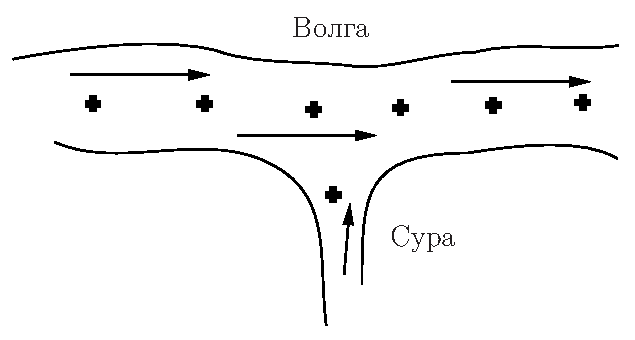
\includegraphics[scale=1]{photo/3.pdf}
	\caption{Схематичная картина Лагранжева и Эйлерова описания. \ding{58} - якорь.}
	\label{fig:figure3}
\end{figure}

\index{Описание!Эйлера}
\paragraph{Эйлерово описание.} Неподвижное пространство заполнено движущейся жидкостью. Движение жидкости будет определено если все величины характеризующую жидкость (скорость движения, давление, плотность, температура и т.д.) \textcolor{red}{будут определены}.
То есть мы следим, как меняются эти величины от точки к точке
\begin{align*} 
\vec{v} &=\vec{v}(\vec{x}, t) \\
T &=T(\vec{x}, t)
\end{align*}
Система заякоренных буев. 
В Эйлеровом описании мы не знаем что делается с отдельной частицей. При этом частные производные от скорости не являются ускорением. Так если течение стационарно и частная производная по времени  равна нулю, частицы в данной точке могут иметь ускорение. Пример – водопад.

Найдем ускорение частицы. За время $ \Delta t $ частица находящаяся в момент времени $t$ в точке с координатами $ x_{k} $ переместится в точку $ x_{k}=x_{k}+\Delta x_{k} $. Тогда для $i$-ой компоненты ускорения имеем
\begin{align*} 
\lim _{\Delta t \rightarrow 0} \frac{\Delta x_{k}}{\Delta t} &=\frac{\partial x_{k}}{\partial t}=v_{k} 
\end{align*}
\begin{align*}
a_{i} &=\lim _{\Delta t \rightarrow 0} \frac{v_{i}\left(x_{k}+\Delta x_{k}, t+\Delta t\right)-v_{i}\left(x_{k}, t\right)}{\Delta t} \\
&=\lim _{\Delta t \rightarrow 0}\frac{\left[v_{i}\left(x_{k}, t\right)+\frac{\partial v_{i}}{\partial x_{k}} \Delta x_{k}+\frac{\partial v_{i}}{\partial t}-v_{i}\left(x_{k}, t\right)\right]}{\Delta t} \\
&=\frac{\partial v_{i}}{\partial x_{k}} v_{k}+\frac{\partial v_{i}}{\partial t} \\
\end{align*}
Таким образом 
\begin{align*} 
a_{i} &=\frac{\partial v_{i}}{\partial t}+v_{k} \frac{\partial v_{i}}{\partial t}=\left(\frac{\partial}{\partial t}+v_{k} \frac{\partial}{\partial t}\right) v_{i} \\
\vec{a} &=\frac{\partial \vec{v}}{\partial t}+(\vec{v}\,\nabla) \vec{v}=\left(\frac{\partial}{\partial t}+(\vec{v}\,\nabla)\right) \vec{v}
\end{align*}

Аналогично находятся и производные от любой другой величины. Эта производная носит название субстанциональной производной.
\begin{align*} 
\frac{d}{d t}=\frac{\partial}{\partial t}+(\vec{v}\,\nabla)
\end{align*}
\subsection{Связь Лагранжева и Эйлерова описаний}
Пусть известно Эйлерово поле скорости $ \vec{v}=\vec{v}(\vec{x}, t) $. Чтобы найти как двигаются Лагранжевы частицы $ \vec{x}(t, \vec{\xi}) $, нам нужно решить уравнение
\begin{align*} 
\frac{d \vec{x}}{d t}=\vec{v}(\vec{x}, t) \\
\vec{x}(t=0, \vec{\xi})=\vec{\xi}
\end{align*}
Как найти эйлерово поле скорости? Если нам известно поведение лагранжевых частиц $ \vec{x}(t, \vec{\xi}\,) $, то вначале нам нужно решить уравнение 
\begin{align*} 
\vec{x}=\vec{x}(t, \vec{\xi})
\end{align*}

Решение этого уравнения 
\begin{align*} 
\vec{\xi}=\vec{\xi}(\vec{x}, t)
\end{align*}
позволяет найти Лагранжеву частицу, которая в момент времени $t$ попала в точку $x$. Тогда эйлерово поле скорости будет равно
\begin{align*} 
\vec{v}(\vec{x}, t)=\vec{v}\qty(t, \vec{\xi}(\vec{x}, t))
\end{align*}

\index{Уравнение!непрерывности}
\index{Закон!сохранения массы}
\subsection{Уравнение непрерывности и закон сохранения массы}
Пусть имеется некоторый объем пространства $V$ заполненный движущейся  жидкостью. Количество жидкости (масса) в этом объеме равно:
\begin{align*} 
m=\int\limits_{V} \rho\dd{V}
\end{align*}
где $\rho$ - плотность жидкости. Жидкость может притекать и вытекать из объема. Введем элемент поверхности $ d \sigma $ и вектор $ \dd \vec{\sigma}=d \sigma \vec{n} $, направленный по внешней нормали к поверхности. 
\begin{figure}[H]
	\vspace{-10pt}
	\centering
	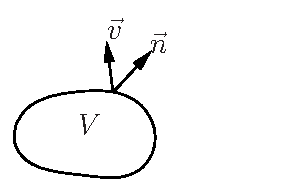
\includegraphics[scale=1]{photo/4.pdf}
	\caption{Объем, скорость и нормаль к поверхности}
	\label{fig:figure4}
\end{figure}
Поток через элемент поверхности определяется скалярным произведением:
\begin{align*}
\oint\limits_{S} \rho \vec{v} d \vec{\sigma}=\int\limits_{V} \Div(\rho \vec{v})\dd{V}
\end{align*}


Уравнение баланса имеет вид:
\begin{align*} 
\frac{\partial}{\partial t} \int\limits_{V} \rho\dd{V}=-\oint\limits_{S} \rho \vec{v} d \vec{\sigma}
\end{align*}
Это интегральный закон сохранения массы. Если на поверхности скорость равна нулю, то масса сохраняется.

Используя формулу Остроградского-Гаусса
\begin{align*} 
\oint\limits_{S} \rho \vec{v} d \vec{\sigma}=\int\limits_{V} \operatorname{div}(\rho \vec{v})\dd{V}
\end{align*}
получим 
\begin{align*} 
\int\limits_{V}\left[\frac{\partial \rho}{\partial t}+\Div(\rho \vec{v})\right]\dd{V}=0
\end{align*}

Так как объем произвольный, то мы получаем дифференциальный закон сохранения
\begin{align*} 
\frac{\partial \rho}{\partial t}+\Div(\rho \vec{v})=0
\end{align*}

Вектор $ \vec{j}=\rho \vec{v} $ - плотность потока массы. Используя формулу $ \nabla(a \vec{b})=\nabla a \vec{b}+a \nabla \vec{b} $, перепишем закон сохранения массы в виде:
\begin{align*} 
\frac{\partial \rho}{\partial t}+(\vec{v}\,\nabla) \rho+\rho \Div(\vec{v})=0 \\
\frac{d \rho}{d t}=-\rho \Div(\vec{v})=0
\end{align*}

\textbf{Несжимаемая жидкость - плотность вдоль траектории частицы не меняется.}
\begin{align*} 
\frac{d \rho}{d t}=0
\end{align*}
То есть поле скорости соленоидально $\Div\vec{v}=0$.

\index{Уравнение!Эйлера}
\subsection{Уравнение Эйлера}
Уравнение движение идеальной жидкости (аналог \textbf{2 закона Ньютона})
Второй закон Ньютона для жидкого элемента
\begin{align*}
\rho\dd{V} \frac{d \vec{v}}{d t} &=\vec{F_{S}}+\vec{F} \\
\vec { F } &= \rho \vec { f }
\end{align*}
Здесь $F$ объемная сила действующая на элемент $dV$ ($f$ – сила отнесенная к единице массы, для силы тяжести $f=g$, где g ускорение свободного падения).

$F_s$ - сила действующая на элемент объема со стороны окружающей среды.  В идеальной среде силы трения нет и единственная сила определяется только силами давления. На элемент поверхности $d\sigma$ действует сила $ P \dd{\vec{\sigma}} $ и результирующая сила равна:
\begin{align*}
\vec { F } _ { S } = - \oint \limits_ { S } p \dd{\vec{\sigma}} = - \int \limits_ { V } \nabla p\dd{V} \approx - \nabla p\dd{V}
\end{align*}

В результате получаем \textbf{уравнение Эйлера}
\begin{align*}
\frac { d \vec { v } } { d t } = - \frac { \nabla p } { \rho } + \vec { f }\,
\frac { \partial \vec { v } } { \partial t } + ( \vec{v}\,\nabla ) \vec { v } = - \frac { \nabla p } { \rho } + \vec { f }
\end{align*}
Здесь мы учли что в уравнение Ньютона входит полная производная. У нас  5 неизвестных – 3 компоненты скорости, давление и плотность. И только 4 уравнения: 3 уравнения Эйлера для трех компонент и уравнение непрерывности.
Нужно еще одно уравнение – уравнение состояния, связывающее давление, плотность и энтропию $S$: $ P = P ( \rho , S ) $ и уравнение для энтропии. Для изоэнтропический жидкости $ \frac {\dd{S} } { d t } = \frac { \partial S } { \partial t } + \vec{v}\,\nabla S = 0 $

Если в начальный момент времени энтропия была одинакова во всем пространстве, то она не будет меняться с течением времени и уравнение состояние принимает вид: $ P = P ( \rho ) $.
В идеальном газе уравнение адиабаты имеет вид (\textbf{уравнение Пуассона}):
\index{Уравнение!Пуассона}
\begin{align*}
P &= P _ { 0 } \left( \rho / \rho _ { 0 } \right) ^ { \gamma } \\
\gamma &= c _ { p } / c _ { v }
\end{align*}
где для идеального газа $\gamma = \frac{i+2}{i}$, ($i$ - количество степеней свободы).
Для жидкостей дело хуже. В разных диапазонах давления имеют разные уравнения состояния. Эмпирическая формула для давления $P$, измеряемого в атмосферах: 
\begin{align*}
\frac { P + B } { 1 + B } = \left( \frac { \rho } { \rho _ { 0 } } \right) ^ { \gamma }
\end{align*}
где $B=3000\text{ атм}$, $\gamma = 7$, давление до $10^5$ атмосфер.

Итак, \textbf{система уравнений для идеальной жидкости} принимает вид:
\begin{align*}
& \frac { \partial \vec { v } } { \partial t } + ( \vec{v}\,\nabla ) \vec { v } = - \frac { \nabla p } { \rho } + \vec { g } \\
& \frac { \partial \rho } { \partial t } + d i v ( \rho \vec { v } ) = 0 \\
& P = P ( \rho )
\end{align*}

\index{Закон!сохранения энергии}
\subsection{Закон сохранения энергии идеальной жидкости}

Энергия единицы объема – кинетическая $+$ внутренняя
\begin{align*}
E = \frac { 1 } { 2 } \rho v ^ { 2 } + \rho \varepsilon
\end{align*}

Закон сохранения энергии в интегральной форме:
\begin{align*}
\pdv{t} \int\limits_{ V } \rho \left( \frac { 1 } { 2 } v ^ { 2 } + \varepsilon \right)\dd{V} = - \oint\limits_{ S } \rho \left( \frac { 1 } { 2 } v ^ { 2 } + \varepsilon \right) \vec { v } \dd{\vec{\sigma}} - \oint \limits_ { S } p \vec { v } \dd{\vec{\sigma}}
\end{align*}

Изменение энергии в объеме равно притоку (выносу) энергии в объем через границы $+$ работа внешних сил давления. Энтальпия равна $ W = \rho \varepsilon + P $ из курса термодинамики и общей физики. Получаем закон сохранения в интегральной форме:
\begin{align*}
\pdv{t} \int \limits_{ V } \rho \left( \frac { 1 } { 2 } v ^ { 2 } + \varepsilon \right)\dd{V} = - \oint \limits_{ S } \rho \left( \frac { 1 } { 2 } v ^ { 2 } + W \right) \vec { v } \dd{\vec{\sigma}}
\end{align*}
По формуле Стокса переходим в правой части от интегрирования по поверхности к интегрированию по объему:
\begin{align*}
\int \limits_{ V } 
\left[ 
	\pdv{t} \rho 
	\qty( \frac{1}{2} v^2 + \varepsilon) + 
	\Div \qty( 
		\rho \qty( 
			\frac{1}{2} v^2 + W 
			) 
		) \vec{v} 
\right] \dd{V} = 0
\end{align*}

Поскольку объем произвольный можно перейти к дифференциальной  форме закона сохранения энергии:
\begin{align*}
& \frac { \partial E } { \partial t } + \Div \vec { N } = 0 \\
& E = \frac { \rho v ^ { 2 } } { 2 } + \rho \varepsilon \\
& \vec { N } = \left[ \frac { \rho v ^ { 2 } } { 2 } + \rho \varepsilon + P \right] \vec { v }
\end{align*}
Здесь $E$ – плотность энергии, $N$ – вектор плотности потока энергии – аналог вектора Пойнтинга в электродинамике. Введён в 1874 году Умовым.

\index{Закон!сохранения импульса}
\subsection{Закон сохранения импульса}
Для единицы объема жидкости импульс равен $ \vec { p } = \rho \vec { v } $. Если закон сохранения энергии мы выводили в интегральной форме, то здесь мы будем стартовать с дифференциальных уравнений. Запишем изменения для $i$-ой компоненты:
\begin{align*}
\pdv{t} \Big( \rho v _ { i } \Big) = \rho \frac { \partial v _ { i } } { \partial t } + v _ { i } \frac { \partial \rho } { \partial t }
\end{align*}

Запишем уравнение Эйлера и уравнение непрерывности по компонентам:
\begin{align*}
\frac { \partial v _ { i } } { \partial t } + \sum _ { k = 1 } ^ { 3 } v _ { k } \frac { \partial v _ { i } } { \partial t } &= - \frac { 1 } { \rho } \frac { \partial P } { \partial x _ { i } } + f _ { i } \\
\frac { \partial \rho } { \partial t } + \sum _ { k = 1 } ^ { 3 } \frac { \partial \left( \rho v _ { k } \right) } { \partial x _ { k } } &= 0
\end{align*}
В результате для изменения компоненты импульса имеем:
\begin{align*}
\pdv{t} \left( \rho v _ { i } \right) = - \frac { \partial } { \partial x _ { k } } \left( P \delta _ { i k } + \rho v _ { i } v _ { k } \right) + \rho f _ { i }
\end{align*}
Здесь по индексу $k$ идет суммирование. Хочется привести это уравнение к дивергентной форме, чтобы получить закон сохранения. Учтем:
\begin{align*}
\rho v _ { k } \frac { \partial v _ { i } } { \partial x _ { k } } + v _ { i } \frac { \partial \left( \rho v _ { k } \right) } { \partial x _ { k } } = \frac { \partial \left( \rho v _ { i } v _ { k } \right) } { \partial x _ { k } }
\end{align*}
Внешние силы приводят к изменению импульса. Нужно что-то придумать с давлением:
\begin{align*}
\frac { \partial P } { \partial x _ { i } } = \frac { \partial \left( \delta _ { i k } p \right) } { \partial x _ { k } }
\end{align*}
Здесь $ \delta _ { i k } = 1 , i = k ; \delta _ { i k } = 0 , i \neq k $ - символ Кронекера.

В результате получим:
\begin{align*}
\pdv{t} \left( \rho v _ { i } \right) = - \frac { \partial } { \partial x _ { k } } \left( P \delta _ { i k } + \rho v _ { i } v _ { k } \right) + \rho f _ { i }
\end{align*}

Введем тензор плотности потока импульса: $ \Pi _ { i k } = P \delta _ { i k } + \rho v _ { i } v _ { k } $. Тогда закон сохранения импульса запишется как:
\begin{align*}
\pdv{t} \left( \rho v _ { i } \right) = - \frac { \partial \Pi _ { i k } } { \partial x _ { k } } + \rho f _ { i }
\end{align*}

Проинтегрируем последнее равенство по объему:
\begin{align*}
\pdv{t} \int \limits_{ V } \rho v _ { i }\dd{V} = - \int \limits_{ V } \frac { \partial \Pi _ { i k } } { \partial x _ { k } }\dd{V} + \int \limits_{ V } \rho f _ { i }\dd{V}
\end{align*}
Используя теорему Остроградского-Гаусса для тензора получаем:
\begin{align*}
\pdv{t} \int \limits_ { V } \rho v _ { i }\dd{V} = - \oint \limits_ { S } \Pi _ { i k } n _ { k } d \sigma + \int \limits_ { V } \rho f _ { i }\dd{V}
\end{align*}
Таким образом, изменение импульса в объеме $V$ связано с потоком импульса через поверхность $S$. Векторная же форма закона сохранения импульса имеем вид:
\begin{align*}
\pdv{t} \int \limits_ { V } \rho  \vec{v}\dd{V}  = - \oint \limits_ { S } [ P \vec { n } + \rho \vec { v } ( \vec { v } \vec{n} ) ]d \sigma
\end{align*}
Здесь $\vec{n}$ - внешняя нормаль.

\paragraph{Следствие.} Как использовать закон сохранения импульса для нахождения силы действия потока на тело? Если движение стационарно:
\begin{align*}
\oint _ { S } \left[ p n _ { i } + \rho v _ { i } v _ { k } n _ { k } \right] d \sigma = 0
\end{align*}
Отсюда для силы действия потока на тело имеем:
\begin{align*}
F _ { i } = - \oint \limits_ { S } p n _ { i } d \sigma = \oint \limits_ { S } \rho v _ { i } v _ { k } n _ { k } d \sigma
\end{align*}
Пример -- изогнутая трубка (душ).
\begin{align*}
\pdv{t} \int \limits_ { V } \rho  \vec{v}\dd{V}  = - \oint \limits_ { S } [ P \vec { n } + \rho \vec { v } ( \vec { v } \vec{n} ) ]d \sigma
\end{align*}
\begin{figure}[H]
	\centering
	\includegraphics[scale=0.6]{example-image-a}
	\caption{картинка изогнутой трубки}
	\label{fig:figure5}
\end{figure}
В одно сечение жидкость втекает, а из другого вытекает.
\subsection{Гидростатика}
Рассмотрим простейший случай когда скорость жидкости равна нулю. Из исходной системы уравнений 
\begin{align*}
& \frac { \partial \vec { v } } { \partial t } + ( \vec{v}\,\nabla ) \vec { v } = - \frac { \nabla p } { \rho } + \vec { f } \\
& \frac { \partial \rho } { \partial t } + d i v ( \rho \vec { v } ) = 0 \\
& P = P ( \rho )
\end{align*}
следует
\begin{align*}
& \nabla P = \rho \vec { f } \\
& P = P ( \rho )
\end{align*}

Пусть внешняя сила потенциальна
\begin{align*}
& \vec { f } = - \nabla u \\
& \nabla P = - \rho \nabla u
\end{align*}
то есть градиенты давления и сила параллельны.

При какой зависимости плотности от координаты последнее уравнение имеет решение? Применим к последнему уравнению операцию ротора
\begin{align*}
& \operatorname { rot } ( \nabla P ) = 0 \\
& \operatorname { rot } ( - \rho \nabla u ) = - \rho \operatorname { rot } ( \nabla P ) - [ \nabla P \nabla \rho ] \\ 
& [ \nabla P \nabla \rho ] = 0
\end{align*}
Таким образом вектора градиентов плотности и потенциала должны быть параллельны.

\emph{Распределение давления в поле тяжести.}
\begin{align*}
& \nabla P = \rho \vec { g } \\
& P = P ( \rho )
\end{align*}
то есть в поле тяжести стационарное решение существует, если плотность зависит от высоты.

Рассмотрим некоторые примеры задач гидростатики.

\paragraph{Жидкость в поле тяжести.} Попросту говоря, простой жизненный пример -- вода в земных условиях.
Плотность постоянна. Ось $z$ направлена вниз.
	\begin{align*}
	& \frac { d P } { d z } = \rho _ { 0 } g \\
	& P = P _ { A } + \rho _ { 0 } g z
	\end{align*}
	Давление увеличивается на 1 атмосферу на 10 метрах.

\paragraph{Изотермическая атмосфера.} Под ней понимается идеальный газ с постоянной температурой $T$. Ускорение можно считать постоянным. Ось $z$ направлена вверх.
	\begin{align*}
	& \frac { d P } { d z } = - \rho ( z ) g \\
	& P = \frac { R } { \mu } \frac { m } { V } T \\
	& P = \frac { R } { \mu } \rho T
	\end{align*}
	Здесь $R$ - универсальная газовая постоянная. $\mu$ - молярная масса газа.
	\begin{align*}
	& \frac { R T } { \mu } \frac { d P } { d z } = - \rho ( z ) g \\
	& \rho = \rho _ { 0 } \exp ( - z / h ) , P = P _ { 0 } \exp ( - z / h ) \\
	& h = \frac { R T } { \mu g }
	\end{align*}
	Здесь $h$ - высота атмосферы, величина порядка 8 км, поэтому изменением силы тяжести можно пренебречь.

\index{Закон!Архимеда}
\paragraph{Закон Архимеда.} На тело, погруженное в жидкость,  со стороны жидкости действует выталкивающая сила, равная весу жидкости, вытесненную этим телом.
	\begin{align*}
	\nabla P = \rho \vec { g }
	\end{align*}
	Сила со стороны жидкости на элемент поверхности $ d \vec { F } = - p \vec { n }\dd{S} $. Здесь $\vec{n}$ - внешняя нормаль. Тогда сила Архимеда равна:
	\begin{align*}
	& \vec { F }_ { A }  = - \oint \limits_ { S } P \vec{n}\dd{S} = - \int \limits_ { V } \nabla P\dd{V} = - \int \limits_ { V } \rho \vec { g }\dd{V} \\
	& \int _ { V } \rho \vec { g }\dd{V} = \vec { P } \approx \rho V \vec { g } \\
	& & \vec { F }_ { A } = - \vec { P }
	\end{align*}
	Здесь $\vec{P}$ - вес вытесненнной жидкости. Причем и плотность, и ускорение \textbf{не обязательно постоянны!}


\subsection{Гидростатическое равновесие. Частота Брента — Вяйсяля}
\index{Частота!Брента-Вяйсаля}
\index{Равновесие!гидростатическое}
Выясним условия, при  которых состояние равновесия жидкости в поле тяжести будет устойчивым.
Будем считать что плотность зависит от глубины. Ось $z$ направлена вниз. Элементарный  объем   находится на глубине $z$, потом $z+x$.

На тело действуют две силы: сила тяжести и сила Архимеда, и в равновесии они равны  по величине:
\begin{align*}
F _ { g } ( z ) &= g \rho ( z ) V _ { 0 } \\
F _ { A } ( z ) &= - F _ { g } ( z ) = - g \rho ( z ) V _ { 0 }
\end{align*}

Пусть данный объем смещается по вертикали на расстояние $x$. Масса сохраняется и сила тяжести не меняется.  Пусть \textbf{жидкость несжимаема}, тогда объем не меняется. А сила Архимеда изменяется, так как плотность вокруг частицы изменилась. Тогда уравнение  Ньютона для объема запишется как:
\begin{align*}
& m \frac { d ^ { 2 } x } { d x ^ { 2 } } = g \rho ( z ) V _ { 0 } - g \rho ( z + x ) V _ { 0 } \\
& m = \rho ( z ) V _ { 0 }
\end{align*}

Разлагая плотность в ряд, и ограничиваясь линейными членами, получаем:
\begin{align*}
\frac { d ^ { 2 } x } { d t ^ { 2 } } = - \frac { g } { \rho } \frac { d \rho } { d z } x
\end{align*}
Это уравнение гармонического осциллятора:
\begin{align*}
& \frac { d ^ { 2 } x } { d t ^ { 2 } } + N ^ { 2 } x = 0 \\
& N ^ { 2 } = \frac { g } { \rho } \frac { d \rho } { d z } \propto \frac { g } { L }
\end{align*}
Здесь $\displaystyle N = \left( \frac { g } { \rho } \frac { d \rho } { d z } \right) ^ { 1 / 2 } $ -- частота Брента-Вяйсаля.
\begin{enumerate}
	\item {\textbf{Устойчивость жидкости} наблюдается при $ N ^ { 2 } > 0 , \frac { d \rho } { d z } > 0$. Элемент совершает колебания с частотой $N$.}
	\item {\textbf{Неустойчивость жидкости} наблюдается при $ N ^ { 2 } < 0 $. Элемент падает вниз или стремится всплыть.}
\end{enumerate}


\subsection{Уравнение Бернулли}
\index{Уравнение!Бернулли}
Получим альтернативную запись уравнения Эйлера в форме Громэка-Лэмба
\begin{align*}
&\frac { \partial \vec { v } } { \partial t } + ( \vec{v}\,\nabla ) \vec { v } = - \frac { \nabla P } { \rho } + \vec { g } \\
&\vec { g } = g \nabla z
\end{align*}
Ось $z$ направлена вниз. Учтем два равенства из курсов векторного анализа и термодинамики(для равновесных обратимых изобарических процессов).
\begin{align*}
&(\vec {v}\, \nabla ) \vec { v } = \frac { 1 } { 2 } g r a d \left( v ^ { 2 } \right) - [ \vec { v } , [\nabla , \vec { v } ]] \\
&\frac { \nabla P } { \rho } = \nabla W \\
&\frac { \nabla P } { \rho } = \nabla \frac { P } { \rho } , \quad \rho = const
\end{align*}

Получаем уравнение Эйлера в форме Громэко-Лэмба
\begin{align*}
\frac { \partial \vec { v } } { \partial t } + \operatorname { grad } \left( \frac { v ^ { 2 } } { 2 } + W - g z \right) = [ \vec { v } , [\nabla , \vec { v }\, ]]
\end{align*}

Рассмотрим частные случаи, получающиеся из уравнения при некоторых условиях.

\subsubsection{Случай стационарного движения}
\index{Движение!стационарное}
В стационарном случае ($\vec{v}=const$) можно выделить два подслучая. Рассмотрим подробнее.

\paragraph{Безвихревое движение.}
\index{Движение!стационарное!безвихревое}
Движение потенциальное, $\operatorname { rot } \vec{v}=0$. 		Тогда из уравнения Громэко-Лэмба имеем
\begin{align*}
& \operatorname { grad } \left( \frac { v ^ { 2 } } { 2 } + W - g z \right) = 0 \\
& \frac { v ^ { 2 } } { 2 } + W - g z = const
\end{align*}
Заметьте, константа в этом случае \textit{сохраняется во всем пространстве.} Если жидкость несжимаема и однородна, то:
\begin{align*}
\frac { v ^ { 2 } } { 2 } + \frac { P } { \rho } - g z = const
\end{align*}
Это уравнение Бернулли для стационарного \textbf{потенциального} движения однородной несжимаемой жидкости.

\paragraph{Вихревое движение.}
\index{Движение!стационарное!вихревое}
Теперь $\operatorname { rot } \vec{v} \neq 0$. 

Введем понятие линии тока. \textbf{Линия тока} - это линия, касательные к которой в данный момент времени и в каждой точке совпадают с вектором скорости $v$.  Линии тока определяются системой дифференциальных уравнений.
\begin{figure}[H]
	\centering
	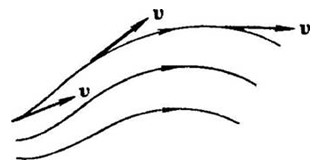
\includegraphics[scale=1]{photo/line.jpg}
	\caption{Линии тока}
	\label{fig:figure6}
\end{figure}
\begin{align*}
\frac { d x } { d v _ { x } } = \frac { d y } { d v _ { y } } = \frac { d z } { d v _ { z } }
\end{align*}
Умножим уравнение Эйлера на вектор скорости, то есть спроектируем на линии тока:
\begin{align*}
& \vec {v}[ \vec { v } , [\nabla , \vec { v } ]]=0 \\
& \vec {v} \perp [ \vec { v } , [\nabla , \vec { v } ]]
\end{align*}
Используя определение линии тока
\begin{align*}
\vec{v}\,\nabla ( \ldots ) = \frac { d } { d l } ( \ldots ) = 0
\end{align*}
получаем тот же закон сохранения
\begin{align*}
\frac { v ^ { 2 } } { 2 } + \frac { p } { \rho } - g z = const
\end{align*}
Но здесь константа сохраняется только вдоль линии тока, и \textit{для разных линий тока константы разные!}

\subsubsection{Случай нестационарного вихревого движения}
\index{Движение!нестационарное вихревое}
\begin{align*}
& \frac { \partial \vec { v } } { \partial t } \neq 0 \\
& \operatorname { rot } v = 0
\end{align*}

В силу потенциальности $ \vec { v } = \nabla \varphi $ из уравнения Громэко-Лэмба получаем
\begin{align*}
\frac { \partial \phi } { \partial t } + \frac { v ^ { 2 } } { 2 } + \frac { p } { \rho } - g z = \mathrm { const }
\end{align*}
Этот интеграл носит название \textbf{интеграла Коши.}

Лучевая трубка тока, трубка образованная множеством линий тока, проходящей через некоторый замкнутый контур.
\begin{figure}[H]
	\centering
	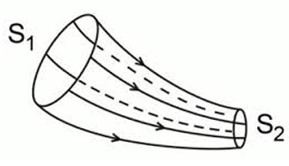
\includegraphics[scale=1]{photo/trubka.jpg}
	\caption{Лучевая трубка}
	\label{fig:figure7}
\end{figure}

\subsubsection{Энергетический смысл уравнения Бернулли}

Закон Бернулли это ничто иное как следствие законов сохранения  массы и энергии вдоль некоторой лучевой трубки через 2 сечения входящее $S_1$ и выходящее $S_2$.

Закон сохранения массы: \textbf{сколько втекает, столько и вытекает.}
\begin{align*}
m _ { i } = \rho _ { i } S _ { i } v _ { i } \Delta t , \quad i = 1,2
\end{align*}
Изменение энергии за счет вытекания и работы силы тяжести равно работе внешних сил:
\begin{align*}
& A _ { i } = p _ { i } S _ { i } v _ { i } \Delta t \\
& E _ { i } = \frac { v _ { i } ^ { 2 } } { 2 } + u _ { i } + \varepsilon _ { i } \\
& A _ { 1 } - A _ { 2 } = \Delta m \left( E _ { 2 } - E _ { 1 } \right)
\end{align*}
Здесь $u$ и $\varepsilon$ - потенциальная и внутренняя энергия. Рассмотрим случай несжимаемой жидкости. В этом случае внутренняя энергия не меняется, а $ u = - g z $. В результате получим уравнение Бернулли.



Уравнение Бернулли имеет множество приложений.
\paragraph{Трубка Пито.}
\index{Трубка Пито}
Знаем сечения, измеряем давления – находим скорости
\begin{align*}
& \frac { v _ { 1 } ^ { 2 } } { 2 } + \frac { p _ { 1 } } { \rho } = \frac { v _ { 2 } ^ { 2 } } { 2 } + \frac { p _ { 2 } } { \rho } \\
& S _ { 1 } v _ { 1 } = S _ { 2 } v _ { 2 }
\end{align*}
\begin{figure}[H]
	\centering
	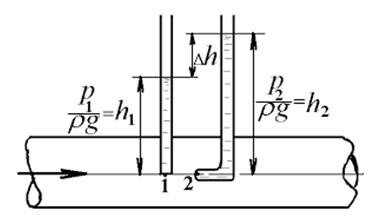
\includegraphics[scale=1]{photo/pito.jpg}
	\caption{Трубка Пито}
	\label{fig:figure8}
\end{figure}


\paragraph{Обтекание двух цилиндров.}
\index{Обтекание!двух цилиндров}
Сближение линий тока, увеличение скорости. Возникает притяжение цилиндров.
\begin{figure}[H]
	\centering
	\includegraphics[scale=0.6]{example-image-c}
	\caption{схематический вид цилиндров}
	\label{fig:figure9}
\end{figure}

\index{Вытекание жидкости}
\paragraph{Вытекание жидкости из сосуда.}
\begin{align*}
& \sigma \ll S \\
& v = \sqrt { 2 g \left( z _ { 1 } - z _ { 2 } \right) }
\end{align*}
\begin{figure}[H]
	\centering
	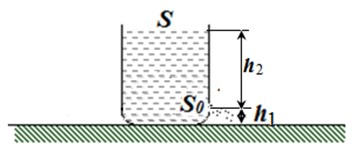
\includegraphics[scale=1]{photo/vutekanie.jpg}
	\caption{Схематичный вид вытекающей жидкости}
	\label{fig:figure10}
\end{figure}

\index{Задача!Прандля}
\paragraph{Задача Прандля.} Эта задача описывает косое падение плоской струи на поверхность и так называемы кумулятивные снаряды. Наряду с уравнением Бернулли нужно использовать закон сохранения импульса.
\begin{figure}[H]
	\centering
	\includegraphics[scale=0.6]{example-image-c}
	\caption{Наклонное падение струи}
	\label{fig:figure11}
\end{figure}
\begin{figure}[H]
	\centering
	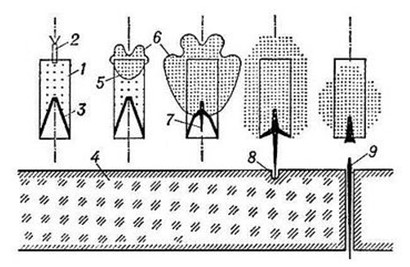
\includegraphics[scale=1]{photo/kommu.jpg}
	\caption{Кумулятивные снаряды}
	\label{fig:figure12}
\end{figure}



\subsection{Теорема Томсона. Потенциальные и вихревые движения жидкости}
\index{Теорема!Томсона}

Введём понятие циркуляции скорости – интеграл, взятый вдоль некоторого замкнутого контура
\begin{align*}
\Gamma = \oint \limits_ { L } \vec { v } \dd{\vec{r}}
\end{align*}
Докажем теорему о сохранении циркуляции скорости – теорему Томсона (лорда Кельвина):
\textbf{Циркуляция скорости вдоль замкнутого контура, перемещающего в идеальной жидкости, остается постоянной.}
\begin{figure}[h]
	\centering
	\includegraphics[scale=0.6]{example-image-c}
	\caption{два контура: начальный и смещенный}
	\label{fig:figure13}
\end{figure}
Выберем замкнутый контур, состоящий из фиксированных частиц (<<жидкий>> контур) и перемещающийся вместе с ними.  Найдем полную производную по времени от этого контура. Происходит изменение как скорости, так и изменение контура во времени
\begin{align*}
\frac{d \Gamma}{d t}=\frac{d}{d t} \oint\limits_{L} \vec{v} d \vec{r}=\oint\limits_{L} \frac{d \vec{v}}{d t} d \vec{r}+\oint\limits_L \vec{v} d\left(\frac{d \vec{r}}{d t}\right)
\end{align*}

Используем определение скорости и уравнение Эйлера
\begin{align*}
\frac { \vec { d v } } { d t } = - \frac { \nabla p } { \rho } - \vec { f }
\end{align*}

Пусть внешняя сила потенциальна, а процесс адиабатический
\begin{align*}
&{ \vec { f } = - \nabla u } \\ 
&{ \frac { \nabla p } { \rho } = \nabla W }
\end{align*}
Здесь $W$ энтальпия.  Учтем, что $ ( \nabla \phi \dd{\vec{r}} ) = d \phi $ и окончательно получим
\begin{align*}
&\frac { d \Gamma } { d t } = \oint _ { l } d \left( \frac { v ^ { 2 } } { 2 } - W - u \right) = 0 \\
& \Gamma = const
\end{align*}

% \begin{itemize}
\paragraph{Следствие 1.} Используем теорему Стокса
\begin{align*}
\oint \limits_ { L } \vec { v } \dd{\vec{r}} = \int \limits_ { S } \vec { n } \operatorname { rot } \vec { v }\dd{S}
\end{align*}
\begin{figure}[h]
	\centering
	\includegraphics[scale=0.6]{example-image-c}
	\caption{Контур и поверхность, натянутая на этот контур}
	\label{fig:figure14}
\end{figure}

Для потенциальных течений $ \operatorname{r o t} \vec { v } = 0 , \Gamma = 0$. Циркуляция скорости по \textbf{односвязанному контуру} в потенциальном течении идеальной жидкости равна нулю.

\paragraph{Следствие 2.} 	Поток вихря через поверхность, натянутую на  \textit{односвязанный контур} в потенциальном течении идеальной жидкости величина постоянная:
	\begin{align*}
	\Gamma = \oint \limits_ { L } \vec { v } \dd{\vec{r}} = \int \limits_ { S } \vec { n } \operatorname{rot}\vec { v }\dd{S} = const
	\end{align*}


\paragraph{Следствие 3.} 
	В потенциальном течении не может быть \textit{замкнутых линий тока} (иначе, взяв ее в качестве контура мы получим, что циркуляция вдоль данного контура не равна нулю).

\paragraph{Следствие 4.} 
	В однородной несжимаемой жидкости можно исключить из рассмотрения уравнений движения давление.  Запишем уравнение Эйлера в форме Громэко-Лэмба
	\begin{align*}
	\frac { \partial \vec { v } } { \partial t } + \nabla \left( \frac { v ^ { 2 } } { 2 } \right) - [ \vec { v } \operatorname{r o t} \vec { v } ] = \nabla ( W + u )
	\end{align*}
	Возьмем от него ротор и учтем, что ротор от градиента равен нулю ($ \operatorname { rot } \nabla \vec { v } = 0 $)
	\begin{align*}
	&{ \pdv{t} \operatorname{r o t} \vec { v } = \operatorname{r o t} [ \vec { v } \operatorname{r o t} \vec { v } ] } \\
	&{\Div \vec { v } = 0 }
	\end{align*}
	Получили полное описание поля скорости с помощью одного уравнения.


% \subsubsection{}
\paragraph{Основные выводы из теоремы Томсона.} Если в какой-то точке линии тока завихренность отсутствует, то она отсутствует и вдоль этой линии.

На первый взгляд отсюда следует:
% \begin{enumerate}
\paragraph{Первый вывод.} Стационарное обтекание любого тела набегающим из бесконечности потоком должно быть потенциальным: $\vec { v } = \text { const }, \,\, \operatorname { rot } \vec { v } = 0$

\paragraph{Второй вывод.} Если движение жидкости потенциально в некоторый момент времени, то оно будет потенциальным и в дальнейшем. В частности:

Потенциальным должно быть всякое движение, при котором в начальный момент жидкость покоилась. В реалии, однако, это этот имеет ограниченную область применимости. Дело в том, что приведенное выше утверждение о сохранении ротора скорости вдоль линии тока неприменимо для линий проходящих воль поверхности твердого тела. Около стенки \textit{нельзя провести односвязный замкнутый контур}. 

Уравнения движения идеальной жидкости допускают решения в которых на поверхности твердого тела, обтекаемого жидкостью твердого тела происходит <<отрыв>> струи: линии тока, следовавшие вдоль поверхности, в некотором месте отрываются от него, уходя в глубь жидкости. Возникает застойная область и на границе течение становится непотенциальным 
\begin{figure}[H]
	\centering
	\includegraphics[scale=0.6]{example-image-c}
	\caption{Обтекание тела с застойными зонами}
	\label{fig:figure14}
\end{figure}
Возникает поверхность <<тангенциального>> разрыва. Скорость терпит разрыв непрерывности.


При учете таких разрывных решений решение уравнений идеальной жидкости неоднозначно: наряду с непрерывным решением появляется бесконечнок множество разрывных решений. При этом разрывные решения не имеют физического смысла: так как тангенциальные разрывы \textbf{абсолютно неустойчивы}, в результате чего движение жидкости становится \textbf{турбулентным}.

Реальное течение безусловно однозначно. Всякая жидкость обладает вязкостью. Малая вязкость практически не проявляется во всем пространстве, но она будет играть определяющую роль в пристеночной области (пограничный слой).

Тем не менее, в ряде случаев это достаточно хорошее приближение.  Например, \textit{хорошо обтекаемые тела}: самолет автомобиль, корабль -- движение жидкости от потенциального отличатся только в области <<пограничного>> слоя и <<следа>> позади тела.

Кроме того, это приближение работает и в случае \textit{малых нестационарных колебаний}. Рассмотрим его подробнее.


\subsubsection{Нестационарные малые колебания}
\index{Колебания!малые нестационарные}
\begin{figure}[H]
	\centering
	\includegraphics[scale=0.6]{example-image-c}
	\caption{Сфера размером $l$ и сфера, смешенная на $a$.}
	\label{fig:figure15}
\end{figure}
$l$ - линейный размер тела, $a$ - характерная амплитуда колебаний, $v$ - скорость колеблющегося тела. Если $l \gg a$, то движение жидкости вокруг тела потенциально. Оценим порядок величины различных членов в уравнении Эйлера
\begin{align*}
\frac { \partial \vec { v } } { \partial t } + ( \vec{v}\,\nabla ) \vec { v } = - \nabla W
\end{align*}
Характерные масштабы изменения скорости $v$ порядка $l$, а изменения скорости во времени определятся частотой колебаний. Оценка членов в уравнении Эйлера
\begin{align*}
\left| \frac { \partial \vec { v } } { \partial t } \right| / \left| \vec{v}\,\nabla ) \vec { v } \right| \propto \frac { u ^ { 2 } } { a } / \frac { l } { u ^ { 2 } } \propto \frac { l } { a } \gg 1
\end{align*}
То есть уравнение Эйлера имеет вид:
\begin{align*}
\frac { \partial \vec { v } } { \partial t } = - \nabla W
\end{align*}
Взяв ротор, имеем:
\begin{align*}
\pdv{t} \operatorname{rot} \vec { v } = 0 , \quad \operatorname { rot } \vec { v } = \operatorname { const } = 0
\end{align*}
Так как при колебательном движении среднее значение по периоду равно нулю.

Таким образом нестационарные \textbf{малые колебания потенциальны}.


\subsection{Потенциальные течения несжимаемой жидкости. Парадокс Даламбера. Присоединенная масса.}
\index{Течение!потенциальное}
\index{Парадокс Даламбера}
\index{Присоединенная масса}

В идеальной баротропной жидкости в поле потенциальных сил вихри не исчезают и не возникают. Если в начальный момент течение было потенциально, то оно будет потенциальным всегда. В ряде случаев это достаточно хорошее приближение, а уравнения гидродинамики существенно упрощаются. 
% \subsubsection{Уравнения гидродинамики несжимаемой идеальной жидкости, когда движение потенциально}
Уравнение непрерывности несжимаемой жидкости:
\begin{align*}
\frac { d \rho } { d t } = 0 ,\quad \Div ( \vec { v } ) = 0
\end{align*}
Поле скорости несжимаемой жидкости соленоидально. Уравнение Эйлера для несжимаемой жидкости:
\begin{align*}
\frac { \partial \vec { v } } { \partial t } + ( \vec{v}\,\nabla ) \vec { v } = - \nabla \frac { p } { \rho } + \vec { g }, \quad \vec { g } = - g \nabla z
\end{align*}
Следовательно
\begin{align*}
\pdv{t} \operatorname { rot } \vec { v } = \operatorname { rot } [ \vec{v} \operatorname { rot } \vec{v}  ]
\end{align*}
то есть движение потенциально. Если сначала движение было потенциально, то и в дальнейшем оно будет потенциальным. Поэтому можно ввести потенциал поля скорости
\begin{align*}
 &\operatorname { rot } \vec { v } = 0 , \quad  { \vec { v } = \operatorname { grad } \varphi } \\  
 &\operatorname { divgrad } \varphi = \Delta \varphi = 0 
\end{align*}
Таким образом, описание потенциального движения идеальной несжимаемой жидкости описывается уравнением Лапласа:
\begin{align*}
\Delta \varphi = 0 , \quad \vec { v } = \operatorname { grad } \varphi
\end{align*}
Для решения этого уравнения также необходимы граничные условия.

\textbf{Условие на протекание}: нормальная компонента скорости жидкости на поверхности тела должна совпадать с проекцией $v_n=\frac { \partial \varphi } { \partial n }=u_n$ скорости самого тела на эту нормаль. \textbf{Второе условие}: обычно используют значение потенциала на бесконечности.

Возникает вопрос: \textbf{как найти давление?} Ответ: из уравнения Бернулли.
\begin{align*}
& \frac { \partial \varphi } { \partial t } + \frac { v ^ { 2 } } { 2 } + \frac { p } { \rho } + u = \operatorname { const } \\
& p = - \left( \frac { \partial \varphi } { \partial t } + \frac { v ^ { 2 } } { 2 } + u \right) + \operatorname { const }
\end{align*}
Константа может зависеть от времени. Для стационарного течения:
\begin{align*}
p = - \left( \frac { v ^ { 2 } } { 2 } + u \right) + \operatorname { const }
\end{align*}

Рассмотрим несколько частных решений уравнения Лапласа(вспомним электростатику)
\begin{itemize}
	\item Пример 1.
	Сдвиговый поток (поле плоского конденсатора), все частицы жидкости двигаются с постоянной скоростью

\end{itemize}





\begin{center}
	\textbf{======Здесь остановился Максим, требуется доделать эту лекцию. Далее Федор, чисто запись лекций в режиме реального времени=======}
\end{center}
\subsection{Гидродинамика плоских течений}
\index{Течение!плоское}
\subsubsection{Аналитические функции}
% Теория аналитических функций задач гидродинамики плоских течений.

У нас есть некоторое комплексное число
\begin{equation}
	z=x+iy 
	\quad \leftrightarrow \quad
	F(z)=\alpha+i \beta
\end{equation}
Функция аналитическая, если независимо от направления стремления $\Delta z$ к нулю существует предел:
\begin{equation}
	F'(z)=\lim\limits_{\Delta z\to0}\frac{F(z+\Delta z)-F(z)}{\Delta z}
\end{equation}
Пример:
\begin{equation}
	F'(z)=\lim\limits_{\Delta x\to0}\frac{\alpha(x+\Delta x,y)+i\beta(x+\Delta x,y)-\alpha(x,y)-i\beta(x,y)}{\Delta x}=
		\pdv{\alpha}{x}+i\pdv{\beta}{x}
\end{equation}
Второй пример:
\begin{equation}
	\Delta z=i\Delta y
\end{equation}
\begin{equation}
	F'(z)=\lim\limits_{\Delta y\to0}\frac{\alpha(x,y+\Delta y)+i\beta(x,y+\Delta y)-\alpha(x,y)-i\beta(x,y)}{i\Delta y}=
		\pdv{\alpha}{y}-\pdv{\alpha}{y}
\end{equation}
Итак, отсюда условие аналитичности
\begin{gather}
	\label{eq2}
	\pdv{\alpha}{x}=\pdv{\beta}{y}, \qquad
	\pdv{\alpha}{y}=-\pdv{\beta}{x}
\end{gather}
Раньше мы вводили потенциал и функцию тока следующим образом:
\begin{gather}
	\label{eq3}
	v_x=\pdv{\phi}{x}=\pdv{\Psi}{y}, \qquad
	v_y=\pdv{\phi}{y}=-\pdv{\Psi}{x}
\end{gather}
Если взять комплексную функцию $F(z)=\phi+i\Psi$ (действительная часть потенциал, мнимая --  функция тока), то это и будет т.н. комплексный потенциал.

Мы помним, что
\begin{gather}
	\nabla^2\phi=0,\quad
	\nabla^2\Psi=0,\quad
	\phi=\Re{F},\quad
	\Psi=\Im{F}
\end{gather}
% Или
% \begin{gather}
% 	\label{eq444}
% 	\phi_1=\Im{F}\\
% 	\Psi_1=\Re{F}
% \end{gather}
\begin{equation}
	v=|F'_z|, \quad
	v=\sqrt{v_x^2+v_y^2}
\end{equation}
Конкретно можно подставлять одну из двух формул для фи и пси.

\subsubsection{Конформное отображение}
Пусть у нас есть функция
\begin{equation}
	z=f(\xi)
\end{equation}
где $z$, $\xi$ -- комплексные. Соответственно
\begin{equation}
	F(z)=F\qty(f(\xi))
\end{equation}

Задачу о цилиндре мы будем решать с помощью конформных отображений: крыло самолета в сечении конформными преобразованиями связано с окружностью. Имея решение об обтекании цилиндра, сможем решить задачу об обтекании крыла самолета. А здесь рассмотрим несколько примеров.

\paragraph{Однородный поступательный поток.} $F(z)=ax+i\cdot ay$, $\phi=ax$, $\Psi=ay$. Что такое линии тока? Это линии $\Psi=\const$. Скорость $v_x=\pdv{\Psi}{x}=a$

\begin{figure}[h!]
    \centering
    \includegraphics[scale=0.5]{example-image-a}
    \caption{Однородный поступательный поток}
    \label{fig:figure1}
\end{figure}
% ---> - линии тока
% 		%B 
% % -----_*->
%  % -|--/|->
%  % -|-/-|-> v_x
%  % -|/--|-> 
% % *_----|->
% % A
% % РИС 1

Задается вопрос на экзамене: у вас есть плоский поток, и вот такая линия по косинусу:

\begin{figure}[h!]
    \centering
    \includegraphics[scale=0.5]{example-image-a}
    \caption{Косинусоидальный профиль}
    \label{fig:figure1}
\end{figure}

\begin{equation}
	Q=\int\limits_{A}^{B} \vec{v}\vec{n}dl=\Psi(B)-\Psi(A)=a(y_b-y_a)
\end{equation}

%--\
% 	\
% 	 \
% 	  \
% 	  |
% 	  |
% 	 /
% 	/
%--/
% Линия по косинусу

\paragraph{Cопряженное течение.} $F(z)=iF(z)=ia-a$:

% -|-|-|->
% -|-|-|->
% -|-|-|->
% Сопряженное течение
\begin{figure}[h!]
    \centering
    \includegraphics[scale=0.5]{example-image-a}
    \caption{Сопряженное течение}
    \label{fig:figure1}
\end{figure}

Дз. Что будут представлять из себя линии тока, если $\alpha=1,\beta=1$? Нужно найти угол наклона.

\paragraph{Cток-исток-вихрь.} У нас в предыдущем разеле было поле конденсатора, поле точечного заряда. В двумерном случае будет потенциал нити.

\begin{equation}
	F(z)=m\ln(z)
\end{equation}

\begin{comment}
     |y
   ______*  
  /     /\
 /     /  \
/     / t  \
-----*--------->x
\          /
 \        /
  \______/
\end{comment}
\begin{gather}
	\label{eqss}
	x=r\cos\theta\\
	y=r\sin\theta\\
	z=x+iy=re^{i\theta}\\
	F(z)=m\ln(re^{i\Theta})=m\ln(r)+mi\theta
\end{gather}
\begin{comment}
Принцип действия логарифмической линейки
 ______________________________________
|_.__.__.___.___.____._____.____.______| ln x
	 ______________________________________
	|_.__.__.___.___.____._____.____.______| шкала произведения
 ______________________________________
|_.__.__.___.___.____._____.____.______| ln y

x*y
x+y

lnx+lny=ln(xy)
\end{comment}

\begin{equation}
	\phi=m\ln{r}, \quad \Psi=m\Theta, \quad v_r=\pdv{\varphi}{r}=\frac{m}{r}
\end{equation}

Линии тока $\Psi=\const$:
\begin{figure}[h!]
    \centering
    \includegraphics[scale=0.5]{example-image-a}
    \caption{Линии тока}
    \label{fig:figure1}
\end{figure}
\begin{comment}
	Тут короче кружочек с радальными стрелочками из центра
\end{comment}

Посчитаем поток. 
\begin{equation}
	Q=\int\limits_{A}^{B} \vec{v}\vec{n}dl=\Psi(B)-\Psi(A)=m(\Theta_b-\Theta_a)
\end{equation}

Давайте честно посчитаем интеграл:
\begin{equation}
	Q=\int\limits_{A}^{B} \vec{v}_r\vec{r}dl=.... % лень писать. Говорят что надо доверять здравому смыслу
\end{equation}

Делаем следующую вещь:
\begin{figure}[h!]
    \centering
    \includegraphics[scale=0.5]{example-image-a}
    \caption{Контур, охватывающий особую точку 0}
    \label{fig:figure1}
\end{figure}
\begin{comment}
окружность, кривулька два раза по окружности:
   ______
  //----\\
 //      \\
//        \\
*          ||
\          //
 \        //
  \______//
  лень
\end{comment}

Проблема была в том, что контур охватывал особую точку $r=0$, И ВСЕ ЭТО НЕ РАБОТАЕТ

\paragraph{Сопряженное течение.}
\begin{equation}
	F(z)=im\ln{z}=im\ln{re^{i \theta}}=im\ln{r}-m\theta
\end{equation}
\begin{equation}
	\phi=m\theta, \quad
	\Psi=m\ln{r}
\end{equation}
Тогда
\begin{equation}
	v_r=\pdv{\phi}{r}=0, \quad
	v_\theta=\frac{1}{r}\pdv{\Psi}{\theta}=\frac{m}{r}
\end{equation}

\begin{figure}[h!]
    \centering
    \includegraphics[scale=0.5]{example-image-a}
    \caption{Линии $\Psi=\const$}
    \label{fig:figure1}
\end{figure}
\begin{comment}
Линии Psi=const   
   ______
  /      \
 /  ._.   \
/  /   \   \
|  |   |   |
\  \._./   /
 \        /
  \______/
\end{comment}

Циркуляция:
\begin{equation}
	\Gamma=\int \vec{v}d\vec{l}=\int \frac{m}{r}\cdot 2\pi r=2\pi m = \const.
\end{equation}
Течение у нас потенциальное. А у потенциального течения циркуляция ноль! Но опять, мы же захватили особую точку в середине, и получили фигню.

Самостоятельно сделать случай $a=\alpha+i\beta$.

$m$ мнимое -- вихрь, действительное -- сток/исток, а нужно сделать для случая $m$ комплексное.

$\alpha>0$ исток (и вихрь), $\alpha<0$ сток (и вихрь). Вихрь из-за беты.

Подставить и решить, как мы делали ранее:
\begin{equation}
	(\alpha+i\beta)\ln{re^{i\theta}}=
		...
\end{equation}

Вообще задача качественно решается в уме. Сходящаяся или расходящаяся спираль.

\paragraph{Гидродинамический диполь.}
\index{Диполь!гидродинамический}
\begin{equation}
	F(z)=-\frac{P}{z}=-\frac{P}{x+iy}=\phi+i\Psi
\end{equation}

\begin{figure}[h!]
    \centering
    \includegraphics[scale=0.5]{example-image-a}
    \caption{Картинка диполя}
    \label{fig:figure1}
\end{figure}
\begin{comment}
	картинка диполя:
     __>___
 \	/ _>__ \ /
  \	|/    \|/
----*      *-------
  / |\_>__/|\
 /	\__>___/ \
\end{comment}

Найдите фи и пси:
\begin{equation}
	\phi=-\frac{Px}{x^2+y^2}, \quad
	\Psi=\frac{Py}{x^2+y^2}
\end{equation}

Линии тока $x^2+y^2=c\cdot y$ -- смещенные окружности.
\begin{equation}
	x^2+y^2-2\frac{1}{2}cy+\frac{1}{4}c^2=\frac{1}{4}c^2 \quad
	x^2+(y-c/2)^2=r^2
\end{equation}
Отсюда $r=\frac{c}{2}$, центр окружности в $(0,c/2)$. Теперь действительно:
\begin{figure}[h!]
    \centering
    \includegraphics[scale=0.5]{example-image-a}
    \caption{Еще диполь}
    \label{fig:figure1}
\end{figure}
\begin{comment}
		   _<_
		  /	  \
		 /	   \
		 \	   /
		  \	o /
------------*----------------->
		 	o
		  /	  \
		 /	   \
		 \	   /
		  \_<_/
\end{comment}

Надо вспомнить, что $\phi=-\frac{Px}{x^2+y^2}$, а $v_x=\pdv{\phi}{x}$. Ну и надо найти скорость, и надо немножко быть ленивым. Чтобы не брать производную от этой функции. Можно взять игрек 0, да и посчитать производную в точке. Ведь линия тока знак везде имеет одинаковый.

\paragraph{Циркуляционное обтекание кругового цилиндра.} У нас имеется 
\index{Обтекание!кругового цилиндра}
\begin{figure}[h!]
    \centering
    \includegraphics[scale=0.5]{example-image-a}
    \caption{Поток, набегающий на цилиндр}
    \label{fig:figure1}
\end{figure}
\begin{comment}
   ______
  /	     /\
 /	   R/  \
/	   /    \
*     *     |  <----------поток набегает на 
\           /
 \         /
  \_______/
\end{comment}
\begin{equation}
	v_r=0, r=R, \quad
	v+x=-v_0, r\to\infty.
\end{equation}

Все просто?
\begin{equation}
	F=F_1+F_2
\end{equation}
$F_1=-v_0z$ -- просто набегает поток
$F_2=-\frac{v_0}{z}-\frac{A}{z}=-v_0r e^{i\theta} -\frac{A}{r} e^{-i\theta}$

Считаем $v_r$:
\begin{equation}
	\pdv{\phi}{r}=-\qty(v_0-\frac{A}{r})\cos\theta
\end{equation}
здесь при $r=R$ $v_r=0$, и мы нашли константу $A=v_0R^2$.
Тогда
\begin{equation}
	F=-v_0\qty(z+\frac{R^2}{z}).
\end{equation}
\begin{figure}[h!]
    \centering
    \includegraphics[scale=0.5]{example-image-a}
    \caption{Обтекание потоком цилиндра}
    \label{fig:figure1}
\end{figure}
\begin{comment}
	   <--\
           \
   ______   \
  /	     /\  \
 /	   R/  \  \
/	   /    \  \_____
*     *     |  <----------поток набегает на 
\           /
 \         /
  \_______/
\end{comment}

\begin{equation}
	F=-v_0\qty(z+\frac{R^2}{z})-\frac{\Gamma i}{2\pi}\ln{z}
\end{equation}

Что такое здесь гамма, во-первых? Посмотрим немножко назад, мы считали циркуляцию по контуру. $\Gamma=m 2\pi$ Вопрос. Граничным условиям удовлетворяет? Мы конструируем решение (в силу линейности уравнения Лапласа), поэтому надо проверять. Проверяем граничные условия. Первые два слагаемых только что проверили. А добавили еще вот такое круговое течение. Добавили условие, что нормальная компонента не изменилась.

Ну давайте найдем, что у нас получится.
\begin{equation}
	v_r=\pdv{\phi}{r}=-v_0\qty(1-\frac{R^2}{r})\cos\theta
\end{equation}
\begin{equation}
	v_\theta\bigg|_{r=R}=2v_0\sin\theta+\frac{\Gamma}{2\pi R}
\end{equation}

Смотрим на поверхность. Что на ней делается. На ней первое слагаемое: у нас обтекает поток, почему скорость в два раза больше? Понятно почему, понятно почему. А вот знак у меня правильный или неправильный? Но это не суть, важно что должен быть минус, проверьте на экзамене, ответ должен быть правильный, а не то что я написал.

Смотрите, цилиндр:
\begin{figure}[H]
    \centering
    \includegraphics[scale=0.5]{example-image-a}
    \caption{Скорости при обтекании}
    \label{fig:figure1}
\end{figure}
\begin{comment}
  2v_0 <--\
           \
   ______   \
  /	     /\  \
 /	   R/  \  \
/	   /    \  \_____
*     *     |  <---------- v_0
\           /
 \         /
  \_______/
\end{comment}
Если мы что-то перекрыли, поток на поверхности больше. Плюсом еще добавилось круговое течение. Что есть? Есть поток, это вот такая картиночка, это одно решение:
\begin{figure}[H]
    \centering
    \includegraphics[scale=0.5]{example-image-a}
    \caption{Обтекание}
    \label{fig:figure1}
\end{figure}
\begin{comment}
       <--\
           \
   ______   \
  /	     /\  \
 /	   R/  \  \
/	   /    \  \_____
*     *     |  <---------- v_0
\           /
 \         /
  \_______/
  (обтекание)
\end{comment}
другое:
\begin{figure}[H]
    \centering
    \includegraphics[scale=0.5]{example-image-a}
    \caption{Вращение вокруг цилиндра по кругу}
    \label{fig:figure1}
\end{figure}
\begin{comment}
  /-----<--\
 /          \
/    ______  \
|   /	   \  \  
|  /	    \  \   
| /	         \  |
| *     *     | |
| \           / |
\  \         / /
 \  \_______/ /
  \__________/  
  (по кругу)
\end{comment}
Следующая картиночка вот какая-то такая
\begin{figure}[H]
    \centering
    \includegraphics[scale=0.5]{example-image-a}
    \caption{Критическая траектория}
    \label{fig:figure1}
\end{figure}
\begin{comment}
	картинка с критической траекторией
\end{comment}
Критическое значение
\begin{equation}
	\Gamma^*=4\Pi v_0 R.
\end{equation}
Если гамма меньше критического, то критическая точка на поверхности цилиндра, если больше, то вне области цилиндра. Идет какая-то сепаратриса:
\begin{figure}[H]
    \centering
    \includegraphics[scale=0.5]{example-image-a}
    \caption{Сепаратриса}
    \label{fig:figure1}
\end{figure}
\begin{comment}
	картинка с сепаратрисой. Студент Иванов построил картинки. Линии уровня.
\end{comment}

Вопрос. Переходим к формуле Жуковского. Что будет делаться с цилиндром? Появится сила или нет, действующая на цилиндр? Появится какая-нибудь сила или нет? Чем надо воспользоваться:
\begin{equation}
	p_0+\frac{\rho v_0^2}{2}=p_s+\frac{\rho v_\theta^2}{2}
\end{equation}
Отсюда
\begin{equation}
	p_s=p_0+\frac{\rho}{2}\qty(v_0^2-v_\theta^2)
\end{equation}
Ну и получается
\begin{equation}
	p_s=p_0+\frac12\rho\qty(v_0^2-4v_0^2\sin^2\theta-\qty(\frac{\Gamma}{2\pi R})^2-\frac{2\Gamma v_0\sin\theta}{\pi R})
\end{equation}
Тогда
\begin{equation}
	F=-\int p\vec{n}d\vec{l}.
\end{equation}

По горизонтали силы никакой нет. Давление больше где скорость меньше, значит оно больше внизу, значит, возникнет подъемная сила. (скорость больше, сложение скорости набегающего потока и кругового).

Чтобы по вертикали посчитать силу, нужно пять слагаемых интегрировать. Не ноль только последнее слагаемое:
\begin{equation}
	F_x=-\int p n_x \dd{l}=\rho \Gamma v_0. 
	% Место на всякий случай
\end{equation}
Это есть формула Жуковского. Интеграл тривиален. Сила пропорциональна плотности, скорости и завихреванности.

Для упражнения вам такой вопрос: у меня есть цилиндр, скатывающийся по наклонной плоскости. (картинка). Одна траектория в вакууме, другая в воздухе. Объяснить какая дальше.

Следующий вопрос. ЧМ по футболу, угловой, мячик, мы ударяем по мячику. Объяснить как бить для сухого листа.

% лекция 22.03.2019
 
% Параграф 2.8. 
\subsubsection{Вихревые движения в идеальной жидкости}\
\index{Движение!вихревое}
До сих пор мы занимались потенциальными течениями: сток исток, двумерное движение и т.д.

Вот введем такую величину (вихрь, завихренность):
\begin{equation}
	\vec\Omega=\Rot \vec{v}
\end{equation}
Ранее мы вводили 
\begin{equation}
	\Gamma=\oint \vec{v} \,\dd\vec{l}
	% по теореме стокса
	=\int_S \Rot \vec{v}\dd \vec{S}=\int_S \vec\Omega\vec{n}\,\dd S 
\end{equation}
Циркуляция скорости по замкнутому контуру равна потоку завихренности.

\begin{figure}[h!]
    \centering
    \includegraphics[scale=0.5]{example-image-a}
    \caption{}
    \label{fig:figure1}
\end{figure}

Теорема Томсона: циркуляция скорости по замкнутому контуру, двигающемуся в идеальной жидкости, постоянна.

Сохраняется постоянным и поток вихря через поверхность, натянутую на контур, $\Gamma=\const$.

Определение: \textit{Вихревая линия - линия, касательная к которой в каждой точке коллинеарна вектору вихря}.

Понятие вихревой трубки. Берем некий первоначальный контур $S$, вдоль каждой точки границы проводим вихревую линию - это будет вихревая трубка:
\begin{figure}[h!]
    \centering
    \includegraphics[scale=0.5]{example-image-a}
    \caption{}
    \label{fig:figure1}
\end{figure}

Теорема Лагранжа. \textit{Элементы идеальной жидкости, лишенные вихрей в начальный момент времени, будут лишены их в дальнейшем.}

Вихри в идеальной жидкости возникнуть и исчезнуть не могут. Чтобы он появился, необходимо взаимодействие с поверхностью, что приводит к неодносвязности контура (мы к этому вернемся), а также непотенциальность сил. Пример непотенциальной силы: заряженная жидкость в магнитном поле.

Посмотрим теорему Лагранжа более аккуратно. 

\begin{figure}[h!]
    \centering
    \includegraphics[scale=0.5]{example-image-a}
    \caption{}
    \label{fig:figure1}
\end{figure}

На поверхности трубки разместим мааленький контур $S_1$. Сосчитаем поток через этот маленький контур: очевидно, он равен нулю 
\begin{equation}
	\Gamma_1=\int \vec\Omega \vec{n}\dd S_1 = 0
\end{equation}

Теперь, если он равен нулю в некий начальный момент, то и в любой момент этот контур будет находится на поверхности этой трубки: так как контур произвольный, представим мысленно трехмерную картинку, что мы берем за кончик контур и немного оттягиваем от трубки. Тогда сразу поток сразу станет не равен нулю. Поскольку контур произвольный, то это означает, что любое малое шевеление с уходом от поверхности приводит к появлению потока. Это доказательство от противного. Это была первая теорема Гельмгольца, о том, что любая линия состоит из одних и тех же элементов жидкости.

Теорема Гельмгольца: \textit{поток вектора вихря через поперечное сечение лучевой трубки остается постоянным}. 

Боковая поверхность лучевой трубки $S_b$

\begin{equation}
 	\int \vec \Omega \vec{n} \dd S=\int_{S_1} \vec \Omega \vec{n} \dd S  + \int_{S_2} \vec \Omega \vec{n} \dd S + \int_{S_b} \vec \Omega \vec{n} \dd S
 \end{equation} 

Очевидно, поток через боковую поверхность равен нулю. Используем формулу Остроградского-Гаусса: интеграл от омеги по поверхности равен интегралу дивергенции омеги по дв:
\begin{equation}
	\int \vec \Omega \vec{n} dS=\iiint \Div\vec \Omega \dd V=0
\end{equation}
Получится
\begin{equation}
	\int_{S_1} \vec \Omega \vec{n} \dd S=\int_{S_2} \vec \Omega \vec{n} \dd S
\end{equation}
Значит, поток постоянный.

Если $\Omega$ можно считать константой, $S$ мало, то $\Omega S$ -- интенсивность вихревой трубки -- ?

\begin{equation}
	\Div \vec{v}=0, \quad
	\vec \Omega=\Rot\vec{v}, \quad
	\pdv{\vec \Omega}{\tau}=\Rot[\vec{v},\vec{\Omega}\,]
\end{equation}

\paragraph{Пример 1: плоское течение.} $\vec{v}=(v_x(y),0,0)$.
\begin{figure}[h!]
    \centering
    \includegraphics[scale=0.5]{example-image-a}
    \caption{Плоское течение}
    \label{fig:figure1}
\end{figure}
 Дивергенция очевидно равна нулю:
\begin{equation}
	\Div\vec{v}=\pdv{v_x}{x}+\pdv{v_y}{y}=0
\end{equation}

Сосчитаем завихренность $\vec\Omega$.

\begin{equation}
	\vec{\Omega}=\mqty| % It's require package "physics"
		\vec{i}&\vec{j}&\vec{k}\\
		\pdv{x}&\pdv{u}&\pdv{z}\\
		v_x&0&0
	|=-\vec{k}\cdot\pdv{v_x}{y}
\end{equation}

Итак, завихренность есть, но она направлена либо на нас, либо от нас по рисунку.

Является ли данное течение стационарным? Когда у нас была гидростатика, мы находили условие равновесия, а потом проверили, будет ли это состояние стационарным. Проверка третьим уравнением, будет.

а) $v_x=b\, y \quad \vec{\Omega}=-b\vec{k}$
б)
\begin{equation}
	v_x(y)=\left\{
	\begin{aligned}
		v_0&, \quad y>0\\
		0&, \quad y<0\\
	\end{aligned}
	\right.
\end{equation}
Это ступенчатая функция:
\begin{equation}
	\vec{\Omega}=\vec{k}\cdot v_0\delta(y)
\end{equation}
Это так называемая вихревая пелена. (рис)

Сосчитаем интеграл тупо по контуру:
\begin{equation}
	\Gamma=lv_0+0+0+0
\end{equation}
С другой стороны,
\begin{equation}
	\Gamma=\int \vec{\Omega}\vec{n}\dd S = lv_0
\end{equation}
Что здесь немного непривычного? Мы привыкли считать, что завихренность  --- это когда что-то крутится. А у нас течение плоско-параллельное, но скорости у разных сечений разные: и у нас движение все равно вихревое.

\paragraph{Пример 1: вращение жидкого цилиндра.} 
\begin{figure}[h!]
    \centering
    \includegraphics[scale=0.5]{example-image-a}
    \caption{Иллюстрация}
    \label{fig:figure1}
\end{figure}
% Цилиндр соосный z, 3d, ось вверх.
\begin{equation}
	v_\theta(r)=\left\{
	\begin{aligned}
		\omega r&, \quad r<R\\
		0&, \quad r>R\\
	\end{aligned}
	\right.
\end{equation}

Здесь можно обойтись формулой попроще. Вектор Омеги направлен по оси $z$, и получается простая формула: 
\begin{equation}
	\Rot\vec{v}=
		\vec\Omega=
		\vec{I}_z \frac{1}{r}\pdv{r}\,rv_\theta=
		\vec{I}_z 2\omega.
\end{equation}
(график линейный в тета от эр)
$r>0$, течение потенциально: $\vec{\Omega}=0$. Считаем, что цилиндр крутится, а течение вокруг него потенциальное.
\begin{equation}
 	\pdv{r} rv_\theta=0 \quad \Rightarrow \quad v_\theta=\frac{A}{r}
 \end{equation} 
Решаем
\begin{equation}
	\Gamma=\int_L \vec{v}\dd\vec{l}=2\pi R\, v_\theta= 2\pi A
\end{equation}
С другой стороны, гамма это поток вихря:
\begin{equation}
	\Gamma=\iint \Rot\vec{v}\vec{n}\dd S =\iint  \Omega_n \dd S = 2\omega\, \pi R^2
\end{equation}
Из этих формул находим
\begin{equation}
	v_\theta=\frac{\omega R^2}{r}=\frac{\Gamma}{2\pi r}
\end{equation}
Ради чего мы все это делали? Надо найти давление:
\begin{equation}
	p+\frac{\rho v^2}{2}=p_0 \quad \Rightarrow \quad
	p=p_0-\frac{\rho v^2}{2}
\end{equation}
Используем уравнение Бернулли, и ищем ошибку, которая здесь была допущена. По формуле получилось на бесконечности и в центре скорость ноль, и давление в центре нуля и на бесконечности одно и тоже. А из опыта известно, что в центре смерча, например, давление пониженное.

Подсказка: использовали уравнение Бернулли, а оно сформулировано в разных случаях: 1) для стационарного потенциального течения во всем пространстве, 2) вдоль лучевой трубки, 3) нестационарное

При $r>R$ можно пользоваться, течение потенциальное. А внутри-то там есть вихрь, течение не потенциально, и формулой Бернулли пользоваться нельзя.

Непонятно как получается такая формула:
\begin{equation}
	r>R: p=p_0-\frac{\rho\omega^2 R^4}{2r^2}
\end{equation}

Внутри пользуемся уравнением Эйлера. Как мы его выводили: масса умножить на ускорение равно силе.
\begin{equation}
	\pdv{v}{t}+\vec{v}\,\nabla\vec{v}=-\frac{\nabla p}{\rho}
\end{equation}
У нас $\pdv{v}{t}=0$. Нужно знать $\vec{v}\,\nabla\vec{v}$ в сферической системе координат. Есть два способа: первый - посмотреть, второй - смотрим на картиночку: частичка движется по окружности, радиус у неё известен $R$, скорость известна $\omega r$. Ускорение центростремительное $a_r=-\frac{v^2}{R}=-\omega^2 r$. Тогда можем записать:
\begin{equation}
	-\omega^2 r  = - \dv{p}{r}\frac{1}{\rho}?
\end{equation}
\begin{equation}
	p(r)=\left\{
	\begin{aligned}
		&p_0-\frac{\rho\omega^2 R^4}{2r^2}&, \quad& r>R\\
		&p_0-\frac{\rho\omega^2 R^4}{2r^2}+\frac{\rho\omega^2 r^2}{2}, \quad& r<R\\
	\end{aligned}
	\right.
\end{equation}
\begin{figure}[h!]
    \centering
    \includegraphics[scale=0.5]{example-image-a}
    \caption{Иллюстрация}
    \label{fig:figure1}
\end{figure}
Получается, что давление в центре маленькое. Чем больше радиус вихря, тем меньше давление.


Если кто-то хочет подумать. Вихрь имеет такую \/ структуру. Попробуйте показать, что в нем есть подъемная сила.


Займемся следующим приближением.
\subsubsection{Точечные вихри}
\index{Вихри!точечные}

Устремляем сечение нашей вихревой трубки к нулю так:
\begin{equation}
	R\to0, \quad \omega\to\infty, \quad \Gamma=2\pi \omega R^2 =\omega A, \quad v_\theta=\frac{\Gamma}{2\pi r}
\end{equation}

Пусть у нас есть много вихрей: 
\begin{figure}[h!]
    \centering
    \includegraphics[scale=0.5]{example-image-a}
    \caption{Много вихрей}
    \label{fig:figure1}
\end{figure}
Как они между собой будут взаимодействовать? У нас есть уравнение Лапласа, которое работает всюду, кроме вихревых линий. Скорость в данной точке равняется суперпозиции скорости от всех вихрей. Дальше, по теореме Гельмгольца, завихренность переносится частицами жидкости. То есть, скорость точечного вихря $\Gamma_i$ равняется скорости жидкости в данной точке, создаваемой всеми остальными вихрями. 

\begin{equation}
	\dv{\vec{r}_i}{t}=\sum\limits_{k\ne i} \vec{v}_k (\vec{r}_i)
\end{equation}

% (чисто техническая картиночка)
\begin{figure}[h!]
    \centering
    \includegraphics[scale=0.5]{example-image-a}
    \caption{Координаты вихря}
    \label{fig:figure1}
\end{figure}
\begin{comment}	
	y
	^
	|
y_i	|- - - - * Г_i
	|   .  ` '
	|._______'_______> x
	         x_i
\end{comment}
\begin{equation}
	r=\sqrt{ (x_k-x_i)^2+(y_k-y_i)^2 }, \quad
	\sin\theta=\frac{y_i-y_k}{r}, \quad v_\theta=\frac{\Gamma_k}{2\pi r_{ik}}
\end{equation}
Первое:
\begin{equation}
	\dv{x_i}{t}=-\frac{1}{2\pi}\sum\limits_{k\ne i} \frac{\Gamma_k (y_i-y_k)}{r^2_{ik}}
\end{equation}
\begin{equation}
	\dv{y_i}{t}=-\frac{1}{2\pi}\sum\limits_{k\ne i} \frac{\Gamma_k (x_i-x_k)}{r^2_{ik}}
\end{equation}
Какие интегралы есть у этой системы?
\begin{equation}
	\sum \Gamma_i\dv{x_i}{t}=-\sum\sum \frac{\Gamma_k\Gamma_i (y_i-y_k)}{r^2_{ik}}=0
\end{equation}
Это значит, что
\begin{equation}
	\sum x_i \Gamma_i=\const=\overline{x}\sum \Gamma_i, \qq{где} \overline{x}=\frac{\sum x_i \Gamma_i}{\sum \Gamma_i}
\end{equation}
Тривиально, что то же самое можно записать по координате $y$. Если $n>2$, других интегралов нету.

Если есть желающие, попробуйте составить программу, которая бы решала эту систему уравнений. Мышкой ставить точку, какая интенсивность гаммы i вводится, мышкой вторая точка ставится интенсивность, и т.д. каждая точка своим цветом, старт, картинки крутятся и вертятся.

Если есть два вихря противоположных знаков, то они уходят на бесконечность: нужно динамическое изменение области просмотра.


Рассмотрим более простую задачу. Всего два вихря: $r_1$ и $r_2$.
\begin{equation}
	\dv{x_1}{t}=-\frac{\Gamma_2 (y_1-y_2)}{2\pi r^2}, \quad r^2=\sqrt{(x_1-x_2)^2+(y_1-y_2)^2}.
\end{equation}
\begin{equation}
	\dv{x_2}{t}=\frac{\Gamma_1 (y_1-y_2)}{2\pi r^2}, \quad r^2=\sqrt{(x_1-x_2)^2+(y_1-y_2)^2}.
\end{equation}
\begin{equation}
	\dv{y_1}{t}=\frac{\Gamma_2 (x_1-x_2)}{2\pi r^2}, \quad r^2=\sqrt{(x_1-x_2)^2+(y_1-y_2)^2}.
\end{equation}
\begin{equation}
	\dv{y_2}{t}=-\frac{\Gamma_1 (x_1-x_2)}{2\pi r^2}, \quad r^2=\sqrt{(x_1-x_2)^2+(y_1-y_2)^2}.
\end{equation}
Домножаем, складываем:
\begin{equation}
	\Gamma_1 x_1 + \Gamma_2 x_2=\const, \quad
	\Gamma_1 y_1 + \Gamma_2 y_2=\const
\end{equation}
Мы нашли два интеграла: центр тяжести не изменяется.
Ну, давайте попробуем еще найти интегралы. Если мы найдем еще два интеграла, то задачу сделаем. Подсказка: из первого уравнения вычесть второе.
\begin{gather}
	\dv{t}\qty(x_1-x_2)=-\frac{\qty(\Gamma_1+ \Gamma_2)}{2\pi}\frac{y_1-y_2}{r},\\
	\dv{t}\qty(y_1-y_2)=\frac{\qty(\Gamma_1+ \Gamma_2)}{2\pi}\frac{x_1-x_2}{r}
\end{gather}
Домножаем, складываем:
\begin{equation}
	(x_1-x_2)\dv{x_1-x_2}{t}+(y_1-y_2)\dv{y_1-y_2}{t}=0 \quad \Rightarrow \quad
	\dv{(x_1-x_2)^2}{t}+\dv{(y_1-y_2)^2}{t}=0
\end{equation}
Отсюда еще один интеграл
\begin{equation}
	(x_1-x_2)^2+(y_1-y_2)^2=r^2=\const	
\end{equation}

Вихри вращаются вокруг неподвижного центра тяжести, с сохранением расстояния между ними. Какие при этом траектории движения? Чтобы найти траекторию, из первого уравнения находим $x_1$, из второго $y_2$, подставляем в это уравнение и получим уравнение окружности.

а) Что же у нас теперь будет? Посмотрим частный случай, когда $\Gamma_2=0$, $\Gamma_1=\Gamma$. (рис) Движение по окружости $v_\theta=\frac{\Gamma}{2\pi r}$, центр тяжести в точке ненулевого вихря.

\begin{figure}[H]
    \centering
    \includegraphics[scale=0.5]{example-image-a}
    \caption{}
    \label{fig:figure1}
\end{figure}

б) Два вихря $\Gamma, \Gamma$ -- центр тяжести посередине, расстояние между вихрями $l$, $v_\theta=\frac{\Gamma}{2\pi l}$.

\begin{figure}[H]
    \centering
    \includegraphics[scale=0.5]{example-image-a}
    \caption{}
    \label{fig:figure1}
\end{figure}

в) Два вихря $\Gamma, -\Gamma$. Центр тяжести будет находится на бесконечности (нетрудно посчитать). $v=\frac{\Gamma}{2\pi l}$. Два таких вихря двигаются с постоянной скоростью.

\begin{figure}[H]
    \centering
    \includegraphics[scale=0.5]{example-image-a}
    \caption{}
    \label{fig:figure1}
\end{figure}

г) Гамма над плоскостью. (рис). Метод изображений даст, что вихри будут двигаться параллельно плоскости.

\begin{figure}[H]
    \centering
    \includegraphics[scale=0.5]{example-image-a}
    \caption{}
    \label{fig:figure1}
\end{figure}

д) Вихрь в угле - как-то параллельно?

\begin{figure}[H]
    \centering
    \includegraphics[scale=0.5]{example-image-a}
    \caption{}
    \label{fig:figure1}
\end{figure}


% Лекция 29.03.
На прошлой лекции для совокупности вихрей:
\begin{gather}
	\label{eqga}
	\dv{\vec{\Gamma_i}}{t}=\sum v_k(\Gamma_i), \quad v_k=\frac{\Gamma_k}{2\pi r_{ik}}
\end{gather}

\subsection{Поверхностные гравитационные волны}
\index{Волны!поверхностные!гравитационные}
К таким волнам относятся карабельные волны, цунами, ветровые волны, внутренние волны в неоднородной жидкости. При исследовании мы будем использовать ряд приближений. Во-первых, жидкость должна быть \textbf{идеальная и несжимаемая} (нет вязкости, звука). Также она должна быть \textbf{однородна} (плотность постоянна). При этом \textbf{поверхность жидкости плоская и неограниченная} (земля в данных масштабах плоская). Кроме того, мы будем рассматривать только волны \textbf{малой амплитуды}.

\begin{figure}[H]
    \centering
    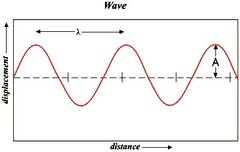
\includegraphics[scale=1.25]{photo/simple_wave.jpg}
    \caption{Характеристики волны}
    \label{fig:simplewave}
\end{figure}

\begin{comment}

       |<------ l ----->|
   ________        ___________
  /        \       /          ^
/           \ _ _ /           | a
------------------------------------------
\end{comment}
\begin{gather}
	\label{eq}
	\pdv{\vec{v}}{t}+(\vec{v},\nabla)\vec{v}=-\frac{\nabla p}{\rho}+\vec{g}
\end{gather}
Оценка:
\begin{gather}
	\label{eq}
	\pdv{v}{t}\sim\frac{V}{\tau}, \quad a\sim V\tau, \quad \tau \sim \frac{a}{V},
	\quad \pdv{v}{t}\sim \frac{v^2}{a}, \quad +(\vec{v},\nabla)\vec{v}\sim \frac{v^2}{l},
	\quad l\gg a
\end{gather}
Значит вторым слагаемым можно пренебречь:
\begin{gather}
	\label{eq}
	\pdv{\vec{v}}{t}=-\frac{\nabla p}{\rho}-\nabla(gz)
\end{gather}
Берем от этого уравнения ротор:
\begin{equation}
	\Rot\Grad=0, \quad
	\Rot\vec{v}=0, \quad \vec{v}=\Grad\phi,
\end{equation}
Из несжимаемости
\begin{equation}
	\Div\vec{v}=0
\end{equation}
Тогда
\begin{equation}
	\nabla^2\phi=0.
\end{equation}
Волны описываются (нет силы тяжести, плотности воды) уравнением Лапласа. 
Давайте подумаем, откуда же что делается. 
Давайте напишем граничные условия.
% \begin{figure}[H]
%     \centering
%     \includegraphics[scale=0.5]{example-image-a}
%     \caption{}
%     \label{fig:figure1}
% \end{figure}

Начнем с поверхности. На поверхности воздух, есть некое давление $p_0$. Можем здесь использовать уравнение Бернулли: вернутся к уравнению Эйлера, вместо скорости вставить градиент фи, получим
\begin{equation}
	\rho\pdv{\phi}{t}+\rho g\xi=-\rho p_0
\end{equation}
Введем смещение волны от плоскости $\xi(x,y)$.

Первое приближение: всегда можем ввести $\phi'=p_0\rho t+\phi$
Второе приближение: возмущения достаточно малы, и получится
\begin{equation}
	\rho\pdv{\phi}{t}+\rho g\xi=0 \quad \bigg|_{z=\xi\approx0}
\end{equation}

Посмотрим, чему равняется вертикальная скорость:
\begin{equation}
	v_z=\dv{\xi}{t}=\pdv{\xi}{t}+\xcancel{(v_z\Grad)\xi}
\end{equation}
Из-за малости колебаний вторым слагаемым пренебрегли:
\begin{equation}
	v_z=\dv{\xi}{t}=\pdv{\xi}{t}
\end{equation}
С другой стороны, 
\begin{equation}
	v_z=\pdv{\xi}{t}=\pdv{\phi}{z}
\end{equation}
Продифференцируем по времени уравнение для $\phi$:
\begin{equation}
	\pdv[2]{\phi}{t}+g\pdv{\phi}{z}=0\bigg|_{z=\xi\approx0}
\end{equation}
Еще нужно граничное условие на дне -- условие непротекания -- вертикальная компонента скорости на дне равна нулю:
\begin{equation}
	\pdv{\phi}{z}=0 \bigg|_{z=-H}
\end{equation}
Если $z\to\infty$, то $\phi \to 0$.

Введем замену $\phi=\Phi(z)\cdot e^{i(kx- \omega t)}$. Тогда
\begin{equation}
	\dv[2]{\Phi}{z}-k^2\Phi=0
\end{equation}
Оно взялось из $\nabla^2\phi=0$. Нам надо найти такое решение, чтобы оно удовлетворяло нулю на дне. 
Решение:
\begin{equation}
	\Phi=A\ch{k(z+H)}
\end{equation}
Тогда
\begin{equation}
	\phi=A\ch{k(z+H)}\cdot e^{i(kx- \omega t)}
\end{equation}
Считаем производные:
\begin{equation}
	\pdv{\phi}{z}=Ak\sh{k(z+H)}\cdot e^{i(kx- \omega t)}
\end{equation}
\begin{equation}
	\pdv[2]{\phi}{t}=-\omega^2A\ch{k(z+H)}\cdot e^{i(kx- \omega t)}
\end{equation}
В итоге получаем дисперсионное уравнение:
\begin{gather}
	-\omega^2A\ch{k(z+H)}\cdot e^{i(kx- \omega t)}+gAk\sh{k(z+H)}\cdot e^{i(kx- \omega t)}=0 \bigg|_{z=0}
	\\ \Rightarrow \quad
	\omega^2=gk\th{kH}
\end{gather}
Вспоминаем:
\begin{equation}
	\th{x}=\frac{e^x-e^{-x}}{e^{x}+e^{-x}}=\frac{\sh x}{\ch x}
\end{equation}

\begin{figure}[H]
    \centering
    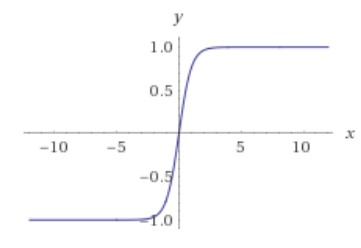
\includegraphics[scale=1]{photo/tanh.jpg}
    \caption{График $\th{x}$}
    \label{fig:figure1}
\end{figure}

У нас есть два масштаба: длина волны $\lambda$ и глубина водоема $H$.

Волны на мелкой воде: $\lambda \gg H$ или $kH\ll 1$.

Получается для волн на мелкой воде
\begin{equation}
	\omega^2=gk^2H, \quad \omega=\pm k\sqrt{gH}
\end{equation}

Волны на мелкой воде -- это волны без дисперсии. Пример яркий волн без дисперсии - это цунами в океане. Глубина океана 5-6 км, а цунами длиной волны десятки, сотни километров.

$v_f=v_{gr}$, если у нас волны на мелкой воде и $v_f=v_{gr}=\sqrt{gH}$.

(оставил парочку строчек)

Второе. $kH \gg 1$. Это волны на глубокой воде. В этом случае тангенс равен 1, и тогда
\begin{equation}
	\omega=\pm\sqrt{gk}
\end{equation}
Волна не чувствует дно, но появляется дисперсия. Примеры волн на глубокой воде -- рябь в луже.

$v_f=\sqrt{\frac{g}{k}}$, $v_{gr}=\frac{g}{2\sqrt{gk}}=\frac12 v_f$.

У нас есть понятие фазовой и групповой скоростей:
\begin{equation}
	v_f=\frac{\omega}{k}=\sqrt{gH}\cdot\sqrt{\frac{\th{kH}}{kH}}, \quad
	v_{gr}=\dv{\omega}{k}=\ldots
\end{equation}

Если у нас есть некий волновой пакет, и мы смотрим как он распространяется, у нас есть огибающая и есть фаза. Групповая скорость - скорость огибающей, фазовая - скорость постоянной фазы.

Нарисуем графики, как выглядит фазовая скорость.

\begin{figure}[H]
    \centering
    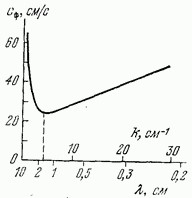
\includegraphics[scale=1.2]{photo/vf.jpg}
    \caption{График фазовой скорости}
    \label{fig:vph}
\end{figure}

\begin{comment}
v_f
^              _
| \           / 
|  \       /
|   \    /
|    \_/
|
|________________________________>l
\end{comment}

На мелкой воде пакет волн двигается вместе, а на глубокой гребни волн будут убегать вперед. Задание к экзамену: оценить время расплывания пакета (рис. \ref{fig:wavelet}) из второй производной
\begin{equation}
	\pdv[2]{\omega}{k} 	
\end{equation} 

\begin{figure}[H]
    \centering
    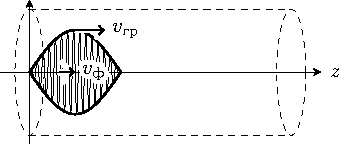
\includegraphics[scale=1.5]{photo/wavelet.pdf}
    \caption{Распространение волнового пакета}
    \label{fig:wavelet}
\end{figure}

Нас интересует, как двигаются частицы. Запишем 
\begin{equation}
	\phi=A\ch{k(z+H)}\cdot\exp(i(kx-\omega t))
\end{equation}

% Частичка находится на некотором горизонте. У нас 
% \begin{equation}
% 	v_x=\pdv{\phi}{x}, \quad v_z=\pdv{\phi}{z}
% \end{equation}
% (потом посчитаем)

% Дальше у нас есть координаты: 
% \begin{equation}
% 	\dv{\xi}{t}=v_x, \quad \dv{\eta}{t}=v_z
% \end{equation}

% В результате мы сможем определить траектории, по которым двигается частица.

% % Лекция 05.04.2019
% % -------------------

% На дне мы задействовали условие непротекания, наверху нестационарное уравнение Бернулли. 

% В результате мы решили уравнение, использовав граничные условия, и получили дисперсионное соотношение.

% \begin{equation}
%     \phi = A \ch{k(z+H)}\exp(i(kx-\omega t)), \quad
%     v = \nabla \phi
% \end{equation}
Мы находимся на некотором горизонте $z$:
\begin{equation}
    v_x = \pdv{\phi}{x} = A\ch{k(z+H)}e^{i(kx-\omega t)}
\end{equation}
\begin{equation}
    v_z = \pdv{\phi}{z} = k\sh{k(z+H)}e^{i(kx-\omega t)} 
\end{equation}
Отсюда
\begin{gather}
    \dv{\xi}{t} = v_x, \quad \xi=\frac{v_x}{-i\omega} = -\frac{kA}{\omega}\ch{k(z+H)e^{(\ldots)}}\\
    \dv{\eta}{t} = v_z, \quad \eta=\frac{v_z}{-i\omega} = \frac{ikA}{\omega}\sh{k(z+H)e^{(\ldots)}} \\
\end{gather}
При $z = 0$ у нас $\xi = a$ (амплитуда на поверхности равна амплитуде колебаний):
\begin{equation}
    a = \xi|_{z = 0} = \frac{ikA}{\omega}\sh{kH}
\end{equation}
Поскольку величины у нас комплексные, мы должны взять действительную часть и получить такой ответ:
\begin{gather}
    \xi = -\frac{a}{\sh{kH}}\ch{k(z+H)}\sin{(kx-\omega t)}\\
    \eta = \frac{a}{\sh{kH}}\sh{k(z+H)}\cos{(kx-\omega t)}\\
\end{gather}
Отсюда видно, что траектории двигаются по эллипсу:
\begin{equation}
    \frac{\xi^2}{a_\xi^2}+\frac{\eta^2}{a_\eta^2} = 1, 
    \quad a_\xi = \frac{a\ch{k(z+H)}}{\sh{kH}}
    , \quad a_\eta = \frac{a\sh{k(z+H)}}{\sh{kH}}
\end{equation}
Надо рассмотреть два случая.


\subsubsection{Волны на мелкой воде}
\index{Волны!поверхностные!на мелкой воде}
В этом случае $kH\ll 1$. Разложим гиперболические функции  в ряд Тейлора при малых аргументах:
\begin{equation}
    \sh{x}\approx x+\ldots, \quad \ch{x}\approx 1+\ldots
\end{equation}
Учтем ещё, что по картинке $k(z+H)$ еще меньше, чем $kH$. Тогда
\begin{equation}
    a_\xi = \frac{a}{kH}, \quad
    a_\eta = a\qty{1+\frac{z}{H}}
\end{equation}

% (картинка с эллипсом и волной)
\begin{figure}[H]
    \centering
    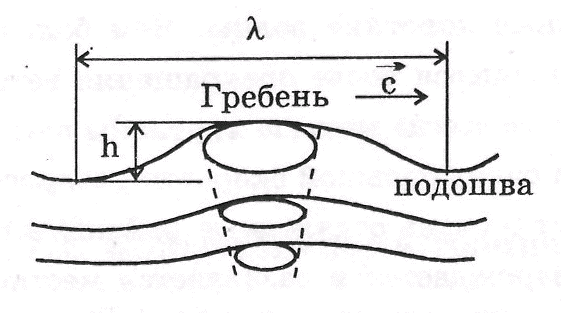
\includegraphics[scale=0.7]{photo/ellipse2.png}
    \caption{Движение частиц на разной глубине}
    \label{fig:ellipse2}
\end{figure}

Частички двигаются по сильно вытянутым траекториям

\subsubsection{Волны на глубокой воде. Волны с сильной дисперсией}
\index{Волны!поверхностные!на глубокой воде}

Теперь $kH\gg 1$. Отбросим некоторые слагаемые по порядку малости. По определению, 
\begin{equation}
    \sh{x} = \frac{e^x+e^{-x}}{2}, \quad \ch{x} = \frac{e^x-e^{-x}}{2}
\end{equation}
Тогда 
\begin{equation}
    \sh{kH}\approx\ch{kH}\approx \frac{e^{kH}}{2} 
\end{equation}
В общем, получится
\begin{equation}
    a_\xi = a_\eta = ae^{kZ}, \quad z<0
\end{equation}
Траектории представляют собой окружности, быстро спадающие с глубиной. 

Займёмся численным экспериментом. 
Оценка такая: мы находимся в море, амплитуда волны $a$ равна пяти метрам.
Это очень серьёзные волны. 
Давайте считать, что длина волны $\lambda$ тоже десять метров, а мы опустились на глубину 10 метров.
Какая будет амплитуда колебания? Если посчитать, то будет один сантиметр. Вот так быстро спадает. Наверху шторм, а на глубине фактически стоит штиль.

\paragraph{Резюме.} Длинные волны -- это волны без дисперсии, траектории продолговатые эллипсы. $v_f = v_{gr} = \sqrt{gH}$. 
\begin{equation}
    \pdv{\xi}{t}+v\pdv{\xi}{x} = 0 ???, \xi = \xi_0(x-vt)
\end{equation}
Выйдем за пределы и будем считать, что
\begin{equation}
    v = \sqrt{g(H+\xi)}
\end{equation}
Попробуйте представить себе, что будет. Волна подходит к берегу, и возникает два эффекта: за счёт малой $H$, энергия то никуда не девается, амплитуда становится больше. Второй эффект в возрастании скорости гребня (быстрее чем подошва), и волны опрокидывается. 

Короткие волны -- это волны с дисперсией, и их траектории -- окружности. При этом $v_f = \frac{\omega}{k} = \ldots$, $v_{gr} = \dv{\omega}{k}$

\subsection{Гравитационно-капиллярные волны}
\index{Волны!поверхностные!гравитационно-капиллярные}
Ранее мы не учитывали поверхностное напряжение. Нарисуем картинку

% (картинка)
\begin{figure}[H]
    \centering
    \includegraphics[scale=0.5]{example-image-a}
    \caption{}
    \label{fig:figure1}
\end{figure}

Есть два главных радиуса кривизны, и возникает избыточное давление:
\begin{equation}
    \delta P = \alpha\qty(\frac{1}{R_1}+\frac{1}{R_2}) = \alpha \frac{1}{R} = -\alpha\nabla \qty(\frac{\nabla\xi}{\sqrt{1+(\nabla\xi)^2}})
\end{equation}
Если $\nabla\xi \sim \frac{a}{\lambda} \ll 1$, то $\delta P_k = -\alpha \Delta \xi$.

Задача свелась к предыдущей. Граничное условие на дне -- не протекание, а на поверхности другое:
\begin{equation}
    \rho\pdv{\phi}{t}+\rho_r g\xi+p_0+\delta P_k = 0, \quad z = 0
\end{equation}
(градиент выкинули в силу линейности задачи, считаем колебания малыми)

От $p_o$ мы легко избавляемся, и в итоге получаем уравнение:
\begin{equation}
    \pdv{\phi}{t}+g\xi+\alpha\Delta\xi = 0 \quad\bigg|_{z = 0}
\end{equation}
Что дальше с этим делать? То же самое, что и раньше. У нас встретились $\phi$ и $\xi$, надо от $\xi$ избавиться. Вспоминаем:
\begin{equation}
    \Delta\xi = \pdv[2]{\phi}{x}
\end{equation}
% ??? 
В результате получаем граничное условие:
\begin{equation}
    \pdv[2]{\phi}{t}+g\pdv{\phi}{z}-\frac{\alpha}{\rho}\frac{\partial^3\phi}{\partial z^2 \partial t} = 0
\end{equation}
Решаем уравнение Лапласа, учитываем граничные условия на дне, и получается следующее решение для потенциала. Теперь подставляем это решение в последнее уравнение, и получаем дисперсионное уравнение
\begin{equation}
    \omega^2 = (gK+\gamma k^3)\th{kH}, \quad \gamma = \frac{\alpha}{\rho}.
\end{equation}
\begin{equation}
    kH \gg 1 \quad \Rightarrow \quad \omega^2 = gK+\gamma k^3.
\end{equation}
Когда же волны существенно капиллярны? Для ряби на воде, например. Понятно, что для цунами этот эффект незначителен. Давайте найдём фазовую скорость:
\begin{equation}
    v_f^2 = \frac{\omega^2}{k^2} = \frac{g}{k}+\gamma k 
\end{equation}
Рисуем график

\begin{figure}[H]
    \centering
    \includegraphics[scale=0.5]{example-image-a}
    \caption{график с минимумом, $\lambda_0 = 1.7 \text{ см}$}
    \label{fig:figure1}
\end{figure}
% (график с минимумом) 

Ищем, чему равен минимум: он равен $k_{*} = \sqrt{\frac{g}{k}}$

\begin{equation}
    v_{gr} = \dv{\omega}{k} \quad \Rightarrow \quad 
    v_{gr} = \frac{v_f}{2}\frac{k_{*}^2+3k^2}{k_{*}^2+k^2}
\end{equation}

При очень маленьких $k$ $v_{gr} = \frac{v_f}{2}$ (как на мелкой воде). 
При больших же $v_{gr} = \frac{3}{2}v_f$.
Итак, у нас есть капиллярные и гравитационные волны.
В одном случае групповая меньше фазовой, в другой больше фазовой. 

\paragraph{Резюме: гравитационные и капиллярные волны.}
Дисперсионное уравнение:
\begin{equation}
    \omega^2 = (gk+\gamma k^3)\th{kH}
\end{equation}
Если $k \gg k_*$, это капиллярные волны. 
Если $\frac{1}{H} \ll k \ll k_*$, то это гравитационные короткие волны (дно ещё не чувствуется).
Если же $k \ll \frac{1}{H}$, то это длинные гравитационные волны.

Попробуем обсудить вот такую задачу:

\begin{figure}[H]
    \centering
    \includegraphics[scale=0.5]{example-image-a}
    \caption{}
    \label{fig:figure1}
\end{figure}
$\rho_0 \gg \rho_1$.

Здесь мы возвращаемся к гидростатике.
Является ли такое состояние решением уравнения гидростатики? (вверху тяжелея, внизу лёгкая).
Гравитация параллельна градиенту плотности, это хорошо. 
А является ли такое состояние устойчивым? 

Нужно написать уравнение Лапласа, поставить граничные условия, написать дисперсионное уравнение с учётом капиллярных сил. 
Считаем, что поверхность достаточно недалеко.

%надо переставить одну спичку
Задача отличается от предыдущей чем?
Перевернули вверх ногами.
Тогда уравнение дисперсии
\begin{equation}
    \omega = \sqrt{-gk+\gamma k^3}
\end{equation}

\begin{figure}[H]
    \centering
    \includegraphics[scale=0.5]{example-image-a}
    \caption{}
    \label{fig:figure1}
\end{figure}

Тут возникают проблемы: отрицательные $\omega^2$. $k_* = \sqrt{\frac{g}{k}}$. Если у вас ка больше ка со звёздочкой (мелкие возмущения), то всё нормально:
\begin{equation}
    \omega_{1,2} = \pm\sqrt{\gamma k^3}
    \quad \Rightarrow \quad
    \xi = c_1e^{i\omega_1 t}+c_2e^{i\omega_2 t}
\end{equation}
А при мнимых омега:
\begin{equation}
    \xi = c_1e^{-|\omega|t}+c_2e^{|\omega|t}
\end{equation}

Итак, при малых возмущениях жидкость просто колеблется,а при больших начинает течь.

Значит, решение устойчивое.
Жизненный пример: перевёрнутый стакан с водой.
Более жизненный -- духи.
Если духи поставить, то хорошие выливаться не будут.
Потому что горлышко узкое, и масштабы маленькие, а ка большое (подавлены крупномасштабные возмущения).
Надо их потрясти: согласно Эйнштейну, движение с ускорением эквивалентно увеличению силы тяжести:
\begin{equation}
    k_{*\text{э}} = \sqrt{\frac{g+a}{k}}
\end{equation}

% Следующий раздел -- внутренние волны/

\subsection{Внутренние волны}
\index{Волны!внутренние}

% Задать малые возмущения, лианеризовать и т.д. Частота Брента-Вейсаля.

% На следующей лекции рассмотрим простую задачу двухслойной жидкости $\rho_1, \rho_2$.
% Ось зет вверх, зададим возмущение на поверхности и надо решить эту задачу.

% Решение ищем в виде бегущей волны, считаем что вверх и вниз убывает (экспоненциально).
% Граничные условия: на границе одинаковая скорость ($\dv{\phi_1}{z} = \dv{\phi_2}{z}$).
% Ещё одно граничное условие -- давление на поверхности: сверху и снизу границы давление одинаково.

% В итоге напишем дисперсионное уравнение. В пределом случае получим гравитационные волны (при $\rho_1 \to 0$).

% 12.04

Итак, у нас такая задача:
\begin{figure}[H]
    \centering
    \includegraphics[scale=0.5]{example-image-a}
    \caption{}
    \label{fig:figure1}
\end{figure}
Считаем, что до границы достаточно далеко.
На границе есть какие-то возмущения
% (рисунок)
\begin{equation}
    \Delta\phi_1 = 0, \quad \Delta\phi_2 = 0
\end{equation}
Справа налево начнём писать уравнение.
Будем искать решение в виде
\begin{gather}
    \phi_1 = A e^{-kz} e^{i(kx-\omega t)}\\
    \phi_2 = B e^{kz} e^{i(kx-\omega t)}
\end{gather}
\begin{equation}
    \phi_1 = \Phi(z)\cdot e^{i(kx-\omega t)}
\end{equation}

Наша задача -- найти дисперсионное уравнение. Займёмся константами. Мы по-прежнему считаем, что колебания относительно малы,
т.е. амплитуда колебаний много меньше длины волны.

Уравнение непрерывности в таком виде (совпадение скоростей на границе):
\begin{equation}
    v_z = (\approx) \pdv{\xi}{t} = \pdv{\phi_1}{z} = \pdv{\phi_2}{z}
\end{equation}
Отсюда сразу следует $B = -A$.

Мы должны поставить второе граничное условие. Используем нестационарное уравнение Бернулли:
\begin{equation}
    p_1 = -\rho_1 g \xi - \rho_1 \pdv{\phi_1}{t}, \quad
    p_2 = -\rho_2 g \xi - \rho_2 \pdv{\phi_2}{t}
\end{equation}
Здесь мы пренебрегли слагаемым $v^2$ в силу малости колебаний.
Граничные условия -- давления на поверхности одинаковы:
\begin{equation}
    kg(\rho_2-\rho_1) = \omega^2(\rho_2+\rho_1)
\end{equation}
Мы избавились от $\xi$ и в итоге получили дисперсионное уравнение:
\begin{equation}
    \omega = \sqrt{gk\frac{\rho_2-\rho_1}{\rho_2+\rho_1}} \approxeq \sqrt{gK\frac{\Delta \rho}{\rho}}
\end{equation}
Предельный случай: $\rho_1 \to 0$ даёт переход к случаю гравитационных волн на глубокой воде. 
В океане $\Delta \frac{\rho}{\rho}\sim 10^{-2}$.

\paragraph{Мертвая вода.} В 1893 г. знаменитый норвежский полярник Фритьоф Нансен, совершавший плавание по арктическим водам, столкнулся со странным явлением. Вот что записал он в отчете: \textit{<<Мы почти не двигались с места ($\ldots$) и будто тащили всю воду за собой. Что мы ни делали, -- круто поворачивали, лавировали, описывали полный круг и пр., -- все напрасно. Лишь только машина переставала работать, судно тотчас же останавливалось, точно схваченное чем-то за корму».}
\index{Мертвая вода}

Явление мертвой воды, обнаруженное Нансеном, заключается в том, что судно на поверхности пресной воды толщиной примерно с судно на соленой воде, тратит всю энергию не на передвижение, а на создание внутренних волн.

Переход к частоте БВ
\begin{equation}
    \pdv{\vec{v}}{t}+(\vec{v}\,\nabla)\vec{v} = -\frac{\nabla p}{\rho}+\vec{g}\\
    \pdv{\rho}{t}+\Div \rho \vec{v} = 0
\end{equation}

Уравнение гидростатики:
\begin{equation}
    \dv{p_0}{z} = -g \rho_0(z)
\end{equation}

\begin{equation}
    \pdv{\vec{v}}{t} = -\frac{\nabla p_0+\nabla p_1}{\rho_0+\rho'}+\vec{g}
\end{equation}

Несжимаемость даст
\begin{equation}
    \dv{\rho}{t} = 0 \quad \Rightarrow \quad
    \Div \vec{v} = 0
\end{equation}

Нетривиальность в следующем: не хватает одного уравнения: переменных 5, уравнений скалярных 4.

Вспомним полную производную:
\begin{equation}
    \pdv{\rho}{t}+\Div \rho \vec{v} = 0
\end{equation}
\begin{equation}
    \pdv{\rho}{t}+(\vec{v}\,\nabla)\rho = 0
\end{equation}
Это записано для возмущений. $\rho = \rho_0+\rho'$:
\begin{equation}
    \pdv{\rho_0}{t}+(\vec{v}\,\nabla)\rho = 0
\end{equation}
\begin{equation}
    (\vec{v}\,\nabla(\rho_0+\rho'))
\end{equation}
Пренебрежём $\vec{v}\,\nabla \rho'$, тогда получим ещё уравнение
\begin{equation}
    \pdv{\rho'}{t}+v_z\dv{\rho_0}{z} = 0
\end{equation}

Вспомним и запишем частоту Брента-Вяйсаля:
\begin{equation}
    N^2 = -g\dv{\rho_0}{z}\frac{1}{\rho_0}
\end{equation}
Тогда последнее уравнение перепишем в виде
\begin{equation}
    \pdv{\rho'}{t}-v_z \frac{N^2}{g}p_0 = 0
\end{equation}
Это уравнение  в \textit{приближении Буссинеска}.

Без всякого вывода рассмотрим один частный случай: экспоненциальная атмосфера, где $\rho_0(z) = \rho_0 e^{-\frac{z}{H}}$, и $N^2 = gH$. 
\begin{equation}
    v_z = A\exp{-i\omega t+ik_xx+ik_zz}
\end{equation}
Здесь $H$ -- эффективная высота атмосферы. Дисперсионное уравнение здесь будет
\begin{equation}
    \omega^2 = N^2\cdot k_x^2
\end{equation}
Можно записать так:
\begin{equation}
    \omega = N\sin\theta, \qq{где} \sin{\theta} = \frac{k_x}{k}
\end{equation}
1) Волны существуют только с частотой $\omega<N$.
2) Зависимость направления от частоты. Если $\omega \to N$, то волновой вектор направлен горизонтально. Если же $\omega \ll N$, напротив, вертикально.
3) $\vec{v_f} \perp \vec{v}_{gr}$:
\begin{figure}[H]
    \centering
    \includegraphics[scale=0.5]{example-image-a}
    \caption{}
    \label{fig:figure1}
\end{figure}

Рисунок с профилем звука в волноводном канале. Из закона сохранения нужно найти закон спадания.
\begin{equation}
   p^2\cdot 2\pi r l \quad \Rightarrow \quad p \sim \frac{1}{r} 
\end{equation}

Попробуем решить такую задачу. В районе Англии произошла катастрофа: взорвались торпеды у подводной лодки. Во сколько раз будет больше акустическое давление в волноводном канале по сравнению с сферической волны? $H \sim 100$ м, мы на побережье Америки. $\sqrt{\frac{l = 5000}{H = 0.1}} \approx 7000$.

\newpage
\section{Движение в вязкой несжимаемой жидкости}

Мы уже столкнулись с рядом парадоксов: парадокс Даламбера -- на тело в потоке жидкости не действует сила. 
Ясно,что это всё не так. Второе -- в жидкости не могут образоваться вихри. Третье -- у нас было граничное условие непротекания:
равенство нулю нормальной компоненты скорости. Но на поверхности неподвижного тела просто скорость равна нулю (опытный факт). 
Парадокс: собирается пыль на поверхности вентилятора, хотя он крутится. Это следствие равенства нулю скорости. 

\subsection{Уравнения гидродинамики вязкой жидкости} %par 3.1
Останется ранее выведенное уравнение. Мы его получили без предположения о не вязкости:
\begin{equation}
    \pdv{\rho}{t}+\Div \rho \vec{v} = 0
\end{equation}
Второе уравнение 
\begin{equation}
    \pdv{\vec{v}}{t}+(\vec{v}\,\nabla)\vec{v} = -\frac{\nabla p}{\rho}+\vec{g}
\end{equation}

Уравнение Эйлера мы вывести смогли, а вот для жидкости вязкой его вывести нельзя. Мы его просто сконструируем.
Рассмотрим такую экспериментальную задачу: у нас есть пластинка на высоте $h$ над нижней (нижняя бесконечная). 
К пластинке площадью $S$ прикладываем силу $F$, и она двигается со скоростью $v$.
Опыт показывает, что чтобы пластинка двигалась с постоянной скоростью, нужно
\begin{equation}
    \frac{F}{S} = \eta \frac{V_0}{h}
\end{equation}
$\eta$ -- это динамический коэффициент вязкости. Для жидкости он убывает с ростом температуры, а для газов медленно растёт.
Можно ввести ещё один коэффициент:
\begin{equation}
    \nu = \frac{\eta}{\rho}.
\end{equation}


%type    eta nu
%Вода 0.01 0.01
%Воздух 1.8\cdot10^{-4}  0.15
%Спирт 0.018    0.022
%Глицерин 8.5   6.8
%Ртуть 0.0156   0.0012
Если мы хотим что-то разогнать, где будет больше? В воздухе.
Будем постепенно переходить к уравнениям. Мысленно выберем в жидкости небольшую площадочку: $\Delta x, \Delta y, \Delta z$.

\begin{figure}[H]
    \centering
    \includegraphics[scale=0.5]{example-image-a}
    \caption{}
    \label{fig:figure1}
\end{figure}

По аналогии можем записать:
\begin{equation}
    \frac{\Delta F}{\Delta S} = \eta \frac{\Delta v_x}{\Delta x}
\end{equation}
Попытаемся сконструировать (но не вывести!) уравнения движения вязкой жидкости.
За основу возьмём закон сохранения импульса:
\begin{equation}
    \pdv{t}\rho v_i = -\pdv{\Pi_{ik}}{x_k}
\end{equation}
Он фундаментален и верен и для вязкой жидкости. А вот ЗСЭ не выполняется: есть трение.

\begin{equation}
    \Pi_{ik} = p \delta_{ik}+\rho v_i v_k+\sigma_{ik}
\end{equation}

Добавили одно слагаемое -- тензор вязких напряжений $\sigma_{ik}$. 
Попробуем его собрать на основе логичных предположений.

Жидкость двигается как целое -- силы трения нет. Она возникает только при смещении слоёв: это первое предположение.
Второе -- мы не рассматриваем экстремальные движения, и считаем что эта зависимость ($\sim \eta$) линейна.
Это линеаризация. Вязкие силы возникают на молекулярных масштабах.
Жидкость будем считать изотропной. Наиболее общий вид тензора вязких напряжений:
\begin{equation}
    \sigma_{ik} = a\qty(
        \pdv{v_i}{x_k}+\pdv{v_k}{x_i}
    )+
    c\qty(
       \pdv{v_i}{x_k}-\pdv{v_k}{x_i}
    )+
    b\sum \pdv{v_i}{x_k} \delta_{ik}
\end{equation}
Если жидкость двигается как целое, силы трения нет. В каких ещё случаях её нет?
Когда жидкость крутится как целое. Это вот что такое:
\begin{equation}
    \vec{v} = [\vec{\Omega}\times \vec{r}\,]  =
    \mqty|
    \vec{i} & \vec{j} & \vec{k}\\
    \Omega_x & \Omega_y & \Omega_z\\
    x& y & z
    |
\end{equation}
Отсюда
\begin{equation}
    v_x = \Omega_y z - \Omega_z y
\end{equation}
% (pass two lines -- for exam)
\begin{equation}
    v_y = \Omega_x z - \Omega_z x, \quad v_z = \Omega_x y - \Omega_y x
\end{equation}

Если честно подставить  в (), получим
\begin{equation}
    \pdv{v_i}{x_k}+\pdv{v_k}{x_i} = 0
\end{equation}
\begin{equation}
    \sum \pdv{v_i}{x_k} \delta_{ik} = 0
\end{equation}

Тогда слагаемое 
\begin{equation}
    \pdv{v_i}{x_k}-\pdv{v_k}{x_i}
\end{equation}
Нулю уже не равно, но при вращении как целого трения нет, значит тензор равен нулю. Значит, коэффициент $c = 0$.

\begin{equation}
    \sum \pdv{v_i}{x_k} \delta_{ik} = 
    \pdv{v_1}{x_1}+\pdv{v_2}{x_2}+\pdv{v_3}{x_3} = \Div \vec{v}
\end{equation}
Оно существенно, когда жидкость сжимаемая. Резюме:
\begin{equation}
    \sigma_{ik}= \eta\qty(
        \pdv{v_i}{x_k}+\pdv{v_k}{x_i}
    )+ \xi\sum \pdv{v_i}{x_k} \delta_{ik}
\end{equation}

% Программа следующей лекции: у нас есть уравнение, выражение для тензора $\Pi_{ik}$, и т.п. Должны получить уравнения Навье-Стокса -- cистема дифференциальных уравнений в частных производных движения вязкой ньютоновской жидкости.

%Лекция от 19.04.2019

Мы взяли за основу уравнение (потому что есть закон сохранения импульса, который выполняется и для вязкой среды):
\begin{equation}
    \pdv{t}\rho v_i = -\pdv{\Pi_{ik}}{x_k}-\sigma_{ik}, \quad 
    \Pi_{ik} = p\delta_{ik} + \rho v_i v_k
\end{equation}
Импульс меняется за счёт сил. Первое слагаемое -- за счёт давления, второе -- за счет (прослушал).
Ещё добавили тензор вязких напряжений $\sigma$. В результате, предполагая что жидкость изотропна
и матрица из 9 элементов симметрична, получаем три константы. После предположения о вращении
жидкости как целого, избавились ещё от одной константы и получили
\begin{equation}
    \sigma_{ik} = \eta \qty(\pdv{v_i}{x_k}+\pdv{v_k}{x_i})+\xi \sum \pdv{v_l}{x_l} v_{k}
\end{equation}
Теперь запишем (используя уравнение непрерывности $\pdv{\rho}{t} = -\pdv{\rho v_k}{x_k}$)
\begin{equation}
    \pdv{\rho}{t}v_i + \rho \pdv{v_i}{t} =  \pdv{t} \rho v_i = \ldots
\end{equation}
Надо суметь продифференцировать эти (?) слагаемые. Это элементарная работа, далее вместо производной плотности 
задействуем уравнение непрерывности.
\begin{equation}
    \pdv{x_k} \rho v_i v_k = v_i \pdv{x_k} \rho v_k + v_k \rho \pdv{v_i}{x_k}
\end{equation}
Замечание:
\begin{equation}
    \pdv{p\delta_{ik}}{x_k} = \pdv{p_k}{x_k}
\end{equation}
В итоге получим
\index{Уравнение!Навье-Стокса}
\begin{equation}
    \rho\qty(
        \pdv{v_i}{t}+v_k\pdv{v_i}{x_k}
    )=
    -\pdv{p}{x_i}+\eta\pdv[2]{v_i}{x_k}+\qty(\frac{\eta}{3}+\xi)\pdv[2]{v_k}{x_i x_k}
\end{equation}
Немножко сгруппировали слагаемые. Это и есть уравнение Навье Стокса, его можно записать в векторной форме:
\begin{equation}
    \rho\qty(\pdv{\vec{v}}{t}+(\vec{v}\,\nabla)\vec{v}) = -\nabla p + \eta \Delta \vec{v} +
   \qty(\frac{\eta}{3}+\xi)\Grad\Div \vec{v}
\end{equation}

Можно ввести коэффициент $\frac{\eta}{\rho} = \nu$, тогда
\begin{equation}
    \pdv{\vec{v}}{t}+(\vec{v}\,\nabla)\vec{v} = -\frac{\nabla p}{\rho}+\nu \Delta \vec{v}
\end{equation}
Размерность 
\begin{equation}
    [\eta] = \frac{L^2}{T}
\end{equation}

Итак, мы получили уравнения Навье-Стокса.

\subsection{Тензор вязких напряжений несжимаемой жидкости}

\begin{equation}
    E_k = \frac{\rho}{2}\int v^2 \dd{V}
\end{equation}
Можно показать, что 
\begin{equation}
    \dv{E_k}{t} = \frac{\rho}{2} \int 2\pdv{v_i}{t} v_i \dd{V}=
    -\frac{\eta}{2} \int   \qty(\pdv{v_i}{x_k}+\pdv{v_k}{x_i})^2 \dd{V}
\end{equation}

Как определять коэффициенты $a, b$, которые мы вводили раньше? Мы конструировали уравнения, не выводя.
Их надо как-то определять экспериментально.

Можно взять круглый диск (касающийся жидкости) на нити, закрутить и определить добротность осциллятора с затуханием. Можно бросить шарик в сосуд. Или прокачивать жидкость через трубу, и скорость вытекания будет как-то зависеть от вязкости.

Рассмотрим такую задачу:

\begin{figure}[h!]
    \centering
    \includegraphics[scale=0.6]{example-image-a}
    \caption{Caption here}
    \label{fig:figure1}
\end{figure}

Верхняя поверхность жёсткая... Рассмотрим стационарный случай:
\begin{equation}
    \pdv{t} = 0
\end{equation}
Кроме того,
\begin{equation}
    \pdv{\Pi_{ik}}{x_k} = 0,\quad
    \Pi_{ik} = p\delta_{ik}+\rho v_i v_k -\sigma_{ik}
\end{equation}
Проинтегрируем это уравнение по внутреннему объёму:
\begin{equation}
    \int_S \Pi_{ik} \eta_k \dd{S} + \int_{S'} \Pi_{ik} \eta_k \dd{S} = 0
\end{equation}
На внутренней поверхности, если жидкость идеальная, то равна нулю нормальная компонента: для вязкой же жидкости равен нулю модуль скорости. Тогда
\begin{equation}
    F_i = -\int p \eta_i \dd{S} - \underbrace{\int \nabla_{ik} \eta_k \dd{S}}_{F'_i}
\end{equation}
У нас есть две силы: первая -- обычное давление, и вязкая сила на единицу поверхности:
\begin{equation}
    f'_i = \sigma_{ik} n_k
\end{equation}
Дурацкий вопрос: скорость равна нулю, а откуда возникает сила? А из равенства нулю скорости не следует равенство нулю градиента.

Будем использовать достаточно часто.

В принципе, мы можем найти силу, с которой жидкость действует на тело, измеряя силу $F'$.

Если каким-то способом удалось измерить скорости и градиенты вдали от тела, то можно по ним найти, чему равна сила.

Должно быть очевидно, что
\begin{equation}
    F_i = F'_i
\end{equation}
(не успел написать почему)

Замечание о граничных условиях.

Твердое неподвижное тело: скорость на поверхности равна нулю.

\begin{figure}[h!]
    \centering
    \includegraphics[scale=0.6]{example-image-a}
    \caption{Caption here}
    \label{fig:figure1}
\end{figure}
\begin{equation}
    \vec{v}= (v_x (y),0,0)
\end{equation}
Наверху жидкости никакой нет, поэтому
\begin{equation}
    f_i = \sigma_{ik} n_k =
    \eta\pdv{v_x}{y} = 0
\end{equation}

\subsection{Течение Куэтта}
\index{Течение!Куэтта}
Плоское течение между двумя пластинками 
\begin{figure}[h!]
    \centering
    \includegraphics[scale=0.6]{example-image-a}
    \caption{Caption here}
    \label{fig:figure1}
\end{figure}

Запишем уравнение Навье-Стокса:
\begin{equation}
    \rho\qty(
        \pdv{v_i}{t}+v_k\pdv{v_i}{x_k}
    )=
    -\pdv{p}{x_i}+\eta\pdv[2]{v_i}{x_k}+f_i
\end{equation}
Начнём упрощать:
\begin{equation}
    \pdv{t} = 0,\quad
    \vec{v} = \qty(v_x (y),0,0), \quad
    p = p(y)
\end{equation}
В этих предположениях 
\begin{equation}
    -\pdv{p}{y} = -g, \quad
    p = p_0 + \rho_0 g y
\end{equation}
Запишем уравнение в проекции на ось ..
\begin{equation}
    \eta\pdv[2]{v_x}{y} = \pdv{p}{y} = 0
\end{equation}
И здесь граничные условия
\begin{equation}
    v_x (0) = 0, \quad
    v_y (H) = V_0
\end{equation}
Будем искать решение в виде $v_x (y) = cy$, тогда
\begin{equation}
    cH = V_0 \quad \Rightarrow \quad c= \frac{V_0}{H}
\end{equation}

Все это было ради силы, мы хотели найти именно её.
\begin{equation}
    f_i = \sigma_{ik} n_k 
\end{equation}
В нашем случае $n_k \equiv n_y = -1$, в таком случае
\begin{equation}
    f_y = -\eta \pdv{v_x}{y}= -\eta \frac{V_0}{H}
\end{equation}
Сила, которая действует на площадку. Умножив её на площадь, получим первую экспериментальную формулу, которую мы получили. Если
бы выводили строго, вместо $\eta$ писали бы некую константу, и
только в конце узнали бы что из эксперимента это $\eta$.

\subsection{Течение Пуазейля}
\index{Течение!Пуазейля}
\begin{figure}[h!]
    \centering
    \includegraphics[scale=0.6]{example-image-a}
    \caption{Caption here}
    \label{fig:figure1}
\end{figure}
Будем рассматривать стационарное течение. Граничное условие
\begin{equation}
    v = v(r), \quad v(R) = 0
\end{equation}
На поверхности трубы у нас скорость равняется нулю. Дальше, 
опять же, возвращаемся к уравнению Навье-Стокса в векторной форме:
\begin{equation}
    \pdv{\vec{v}}{t}+(\vec{v}\,\nabla)\vec{v} = 
    - \frac{\nabla p}{\rho}+\nu \Delta \vec{v}
\end{equation}
В левой части стоит ускорение. У нас частички все двигаются по прямой с постоянной скоростью, значит, скорость и градиент будут со направлены и скалярное произведение ноль. Значит, вся левая часть обращается в нуль. Считаем, что внешних сил никаких нет, тогда получаем уравнение (вспомним, что $\nu = \frac{\eta}{\rho}$
\begin{equation}
    \pdv{p}{z} = \eta 
   \qty[
   \frac{1}{r} \pdv{r} r \pdv{v}{r}
   ]
\end{equation}
Отсюда первое тривиальное заключение
\begin{equation}
    \pdv{p}{z} = c_1
\end{equation}
Тогда
\begin{gather}
    \eta\frac{1}{r} \pdv{r} r \pdv{v}{r} = a_1
    \quad \Rightarrow \quad
    \eta r\pdv{v}{r} = c_1 \frac{r^2}{2} + c_{1}\\
    v = \qty(\dv{p}{z}) \frac{r^2}{4\eta}+A \ln(r) + B
\end{gather}
Из физической реализуемости $A = 0$, а из условия
\begin{equation}
    v(R) = 0 \quad \Rightarrow \quad
    v(r) = \qty(\dv{p}{z}) \frac{1}{4\eta}\qty(r^2-R^2)
\end{equation}

Если вода бежит вправо, то слева давление больше, и градиент скорости отрицательный. Тогда профиль скорости будет таким:

\begin{figure}[h!]
    \centering
    \includegraphics[scale=0.5]{example-image-a}
    \caption{Caption here}
    \label{fig:figure1}
\end{figure}

Сосчитаем поток:
\begin{equation}
    Q=2\pi \int\limits_0^R v(r) r \dd{r} =
    \frac{\pi}{8\eta} \qty(\pdv{p}{z})\cdot R^4
\end{equation}
Там, где самая большая скорость (в центре), элемент площади при интегрировании очень мал. Поэтому получается такая зависимость.

Что будет, если в трубу вставить ещё одну трубу? Останется константа $A$, исчезнет нерегулярность логарифма. Придётся ставить два граничных условия, на обеих трубах.

Ещё может быть, что внутренний диаметр трубы стремится к нулю. Какой будет при этом профиль? Нужно сделать аккуратно предельный переход.

Последний комментарий по этой задаче -- найдём силу:
\begin{equation}
    f_z = \eta_{ik} n_k = -\sigma_{zr} = -\eta \pdv{v_r}{r}=
    -\frac{1}{2} \qty(\dv{p}{z})R
\end{equation}

\newpage
\subsection{Нестационарное движение вязкой жидкости. Вязкие волны}
\index{Волны!вязкие}

Постановка задачи такая: у нас гармонически колеблется пластинка, сверху имеется жидкость. Как она будет колебаться?
\begin{figure}[h!]
    \centering
    \includegraphics[scale=0.5]{example-image-a}
    \caption{Caption here}
    \label{fig:figure1}
\end{figure}
Запишем уравнение Навье-Стокса для несжимаемой жидкости (из соображений симметрии $\vec{v}=(v_x (z),0,0)$, очевидно):
\begin{gather}
    \Div \vec{v} = 0 \quad \Rightarrow \quad \pdv{v_z}{z} = 0\\
    \pdv{v_x}{dt} = \nu \pdv[2]{v_x}{z}
\end{gather}
Будем искать решение в виде 
\begin{equation}
    v_x = A e^{i\omega t + ikz}
\end{equation}
Тогда
\begin{equation}
    -i \omega = \nu k^2 \quad \Rightarrow \quad
    k = (1+i) \sqrt{\frac{\omega}{2\nu}}
\end{equation}
Можно ввести величину
\begin{equation}
    \delta=\sqrt{\frac{2\nu}{\omega}}
\end{equation}
Это толщина скин-слоя. 
